% =====================================================================
%  CONCISE STUDY GUIDE
%  Per-site retrieval of lunar regolith thermal conductivity K_d at the
%  Apollo 15 & 17 heat-flow boreholes.
%
%  A 30-40 page study guide. Three things only: the pipeline, the slope
%  method (flux-anchored equilibrium), and how it differs from brute force.
%  The full 83-page reference is archived in reference/guidebook-extended.tex.
%
%  Self-contained for Overleaf: upload this folder (guidebook.tex + figures/).
%  Compile:  latexmk -pdf guidebook.tex
% =====================================================================
\documentclass[11pt]{report}

\usepackage[a4paper,margin=2.2cm]{geometry}
\setlength{\emergencystretch}{3em}
\raggedbottom
\setlength{\parskip}{2pt plus 1pt minus 0.5pt}
\setlength{\intextsep}{10pt plus 3pt minus 2pt}
\setlength{\floatsep}{10pt plus 3pt minus 2pt}
\setlength{\textfloatsep}{12pt plus 4pt minus 2pt}
\setlength{\abovecaptionskip}{6pt}
\setlength{\belowcaptionskip}{3pt}
\renewcommand{\topfraction}{0.9}
\renewcommand{\bottomfraction}{0.9}
\renewcommand{\textfraction}{0.1}
\setcounter{topnumber}{3}
\setcounter{bottomnumber}{3}
\usepackage[T1]{fontenc}
\usepackage{newtxtext,newtxmath}
\usepackage[scaled=0.90]{helvet}
\usepackage{microtype}
\usepackage{amsmath}
\usepackage{graphicx}
\usepackage{booktabs}
\usepackage{array}
\usepackage{xcolor}
\usepackage{listings}
\usepackage[most]{tcolorbox}
\usepackage{enumitem}
\setlist{topsep=2pt,itemsep=1pt,parsep=0pt}
\usepackage{titlesec}
\usepackage{fancyhdr}
\usepackage[hidelinks]{hyperref}
\usepackage{tikz}
\usetikzlibrary{positioning, arrows.meta, calc, fit, backgrounds}

% ---- palette ----
\definecolor{forest}{HTML}{3D6E4A}
\definecolor{coral}{HTML}{B85B3A}
\definecolor{teal}{HTML}{2C6E73}
\definecolor{char}{HTML}{2B2B2B}
\definecolor{dim}{HTML}{6B6B6B}
\definecolor{rulec}{HTML}{C9C2B6}
\definecolor{codebg}{HTML}{F4F2EE}
\definecolor{codekw}{HTML}{3D6E4A}
\definecolor{codestr}{HTML}{B85B3A}
\hypersetup{colorlinks=true,allcolors=teal}

% ---- headings ----
\titleformat{\chapter}[hang]{\normalfont\sffamily\LARGE\bfseries\color{forest}}
  {\thechapter.}{0.5em}{}
\titleformat{\section}{\normalfont\sffamily\large\bfseries\color{forest}}{\thesection}{0.6em}{}
\titleformat{\subsection}{\normalfont\sffamily\bfseries\color{char}}{\thesubsection}{0.5em}{}
\titlespacing*{\chapter}{0pt}{12pt}{6pt}
\titlespacing*{\section}{0pt}{8pt}{3pt}
\titlespacing*{\subsection}{0pt}{6pt}{2pt}

\pagestyle{fancy}\fancyhf{}
\renewcommand{\headrulewidth}{0.4pt}
\fancyhead[L]{\sffamily\footnotesize\color{dim}Apollo $K_d$ --- study guide}
\fancyhead[R]{\sffamily\footnotesize\color{dim}\thepage}

% ---- code listings ----
\lstdefinestyle{py}{language=Python, basicstyle=\ttfamily\footnotesize\color{char},
  backgroundcolor=\color{codebg}, frame=single, framerule=0pt, rulecolor=\color{rulec},
  keywordstyle=\color{codekw}\bfseries, commentstyle=\color{dim}\itshape,
  stringstyle=\color{codestr}, showstringspaces=false, breaklines=true,
  columns=fullflexible, xleftmargin=8pt, aboveskip=4pt, belowskip=2pt,
  literate={->}{{$\rightarrow$}}2 {**}{{$^{\wedge}$}}1}

\newcommand{\Tm}{\langle T\rangle}
\newcommand{\code}[1]{{\ttfamily\small #1}}

% ---- callout boxes ----
\newtcolorbox{plain}[1][]{colback=teal!6,colframe=teal!55,boxrule=0.6pt,arc=2pt,
  left=6pt,right=6pt,top=3pt,bottom=3pt,before skip=4pt,after skip=4pt,
  title={\sffamily\bfseries In plain words},coltitle=teal,fonttitle=\small,#1}
\newtcolorbox{keypt}[1][]{colback=forest!7,colframe=forest!55,boxrule=0.7pt,arc=2pt,
  left=6pt,right=6pt,top=3pt,bottom=3pt,before skip=4pt,after skip=4pt,
  title={\sffamily\bfseries Key point},coltitle=forest,fonttitle=\small,#1}
\newtcolorbox{warn}[1][]{colback=coral!8,colframe=coral!70,boxrule=1pt,arc=2pt,
  left=6pt,right=6pt,top=3pt,bottom=3pt,before skip=4pt,after skip=4pt,
  title={\sffamily\bfseries Warning},coltitle=coral,fonttitle=\small,#1}
\newtcolorbox{stepbox}[2][]{colback=forest!5,colframe=forest!40,boxrule=0.6pt,arc=2pt,
  left=6pt,right=6pt,top=3pt,bottom=3pt,before skip=4pt,after skip=4pt,
  title={\sffamily\bfseries #2},coltitle=forest,fonttitle=\small,#1}
% A description box that sits below a figure.  Keeps the longer read off
% the data area of the figure itself.
\newtcolorbox{figdesc}{colback=teal!4,colframe=teal!25,boxrule=0.4pt,arc=2pt,
  left=6pt,right=6pt,top=4pt,bottom=4pt,before skip=2pt,after skip=8pt,
  fontupper=\small\itshape\color{char}}

\begin{document}

% ================= TITLE =================
\thispagestyle{empty}
\begingroup\color{forest}\hrule height 2.5pt\endgroup
\vspace{8pt}
{\sffamily\bfseries\color{forest}\LARGE Per-site retrieval of lunar regolith\\[2pt]
thermal conductivity $K_d$ at the Apollo 15 \& 17\\[2pt]
heat-flow boreholes\par}
\vspace{6pt}
{\sffamily\Large\color{char} A study guide: the pipeline, the slope method, and how it differs from brute force\par}
\vspace{6pt}
{\color{dim}\large A concise companion to the JGR letter.\par}
\vspace{4pt}
{\color{char} R.\,P.\ Gregorio \quad\textbullet\quad Kasai Laboratory, Institute of Science Tokyo}
\vspace{6pt}
\begingroup\color{rulec}\hrule height 1pt\endgroup
\vspace{8pt}

\begin{abstract}
\noindent
We measure how well heat conducts through the deep lunar regolith --- the
parameter $K_d$ --- separately at the Apollo~15 and Apollo~17 heat-flow
boreholes, and find them to differ by about a factor of two
($K_{d,\mathrm{A15}}^{*}=4.58$, $K_{d,\mathrm{A17}}^{*}=8.12$
mW\,m$^{-1}$\,K$^{-1}$). This guide explains the three things that matter and
nothing else: the \textbf{pipeline} that turns raw Apollo thermometer records
into one number per site (Ch.~\ref{ch:pipeline}); the \textbf{slope method} ---
the flux-anchored equilibrium solver that is the methodological contribution of
this work (Ch.~\ref{ch:slope}); and \textbf{how that method differs} from the
brute-force spin-up it replaces (Ch.~\ref{ch:bruteforce}). It closes with the
result and how to reproduce it. Read it straight through in about ninety
minutes; you should come out able to explain both the pipeline and the slope
method to someone else.
\end{abstract}

\vspace{4pt}
\tableofcontents
\clearpage

% ================= NOTATION =================
\chapter*{Symbol reference}
\addcontentsline{toc}{chapter}{Symbol reference}
\markboth{Symbol reference}{Symbol reference}
\noindent Every symbol used in this guide, with where its value comes from ---
a measurement, a published model, or a derivation here. $K_d$ (boxed) is the one
number we retrieve.

\begin{center}\footnotesize
\begin{tabular}{@{}p{1.7cm}p{5.4cm}p{3.0cm}p{4.8cm}@{}}
\toprule
Symbol & Meaning & Units / value & Source \\
\midrule
$z,\;t,\;T$ & depth, time, temperature & m, s, K & the axes \\
$K(T,z)$ & thermal conductivity & W\,m$^{-1}$\,K$^{-1}$ & Hayne (2017), Eq.~\eqref{eq:Khayne} \\
$K_c(z)$ & contact (non-radiative) part of $K$ & --- & Hayne (2017), Eq.~\eqref{eq:Kc} \\
$K_s$ & surface contact conductivity & $0.74\times10^{-3}$ & Hayne (2017), fixed \\
$\boxed{K_d}$ & \textbf{deep contact conductivity} & retrieved & \textbf{the answer} \\
$H$ & compaction $e$-folding depth & 0.06 m & Hayne (2017), fixed \\
$\chi$ & radiative enhancement coefficient & 2.7 (cf.\ 1.48) & Hayne (2017), fixed \\
$T_{\rm ref}$ & radiative reference temperature & 350 K & Hayne (2017) \\
$\rho(z),\,c_p(T)$ & density, specific heat & kg\,m$^{-3}$, J\,kg$^{-1}$K$^{-1}$ & Hayne (2017); Hemingway (1973) \\
$\kappa$ & thermal diffusivity $K/(\rho c_p)$ & $\sim10^{-8}$ m$^2$\,s$^{-1}$ & derived \\
$A,\;\varepsilon$ & Bond albedo, emissivity & 0.131/0.137,\; 0.95 & Hayne (2017); code constant \\
$S(t)$ & incident solar flux at surface & W\,m$^{-2}$ & cosine forcing in code \\
$T_s$ & surface skin temperature & K & Newton solve, surface BC \\
$P$ & synodic lunation period & 29.53 d & ephemeris \\
$\delta$ & thermal skin depth $\sqrt{2\kappa/\omega}$ & $\sim$0.04--0.10 m & derived \\
$Q_b$ & basal geothermal heat flux & 21 / 15 mW\,m$^{-2}$ & Langseth (1976), fixed \\
$z_0$ & reconstruction anchor depth & 0.25 then 0.55 m & code constant \\
$u_{\rm rect}$ & rectified (eddy) flux correction & W\,m$^{-2}$ & derived (\S\ref{sec:closure}) \\
$\Tm$ & cycle-mean temperature profile & K & solver output \\
$T_{\rm eq}$ & per-sensor equilibrium temperature & K & stable-window mean of HFE \\
$N$ & number of deep sensors & 7 / 16 & $z>80$\,cm cut (Nagihara 2018) \\
RMSE & deep-sensor misfit & K & Eq.~\eqref{eq:rmse} \\
$\boxed{K_d^*}$ & \textbf{best-fit deep conductivity} & 4.58 / 8.12 & minimum of the RMSE curve \\
$p$ & contrast bootstrap $p$-value & 0.011 & \S\ref{sec:resultstats} \\
\bottomrule
\end{tabular}
\end{center}

\vspace{4pt}
\noindent\textbf{Introduced in the derivations} (App.~\ref{app:deriv})
\begin{center}\footnotesize
\begin{tabular}{@{}p{1.7cm}p{5.4cm}p{3.0cm}p{4.8cm}@{}}
\toprule
Symbol & Meaning & Units / value & Source \\
\midrule
$q$ & conductive heat flux $-K\,\partial_z T$ & W\,m$^{-2}$ & Fourier's law (App.~\ref{app:heateq}) \\
$K_{i+1/2}$ & harmonic-mean face conductivity & W\,m$^{-1}$K$^{-1}$ & App.~\ref{app:grid} \\
$C_i$ & cell heat capacity $\rho c_p\,\Delta z_i$ & J\,m$^{-2}$K$^{-1}$ & finite-volume cell \\
$g$ & grid growth ratio per cell & 0.08 & \code{config.py}, \code{GRID} \\
$\theta$ & time-weighting of the $\theta$-method & $\tfrac12$ for CN & App.~\ref{app:cn} \\
$r$ & diffusion number $\kappa\,\Delta t/\Delta z^2$ & --- & von Neumann analysis \\
$\xi$ & per-step amplification factor & $|\xi|\le1$ (stable) & von Neumann analysis \\
$k$ & Fourier mode wavenumber & m$^{-1}$ & von Neumann analysis \\
$a_i,b_i,c_i,d_i$ & tridiagonal sub/diag/super/RHS & --- & App.~\ref{app:assembly} \\
$R(T_s),\,R'(T_s)$ & surface residual and its derivative & --- & App.~\ref{app:newton} \\
\bottomrule
\end{tabular}
\end{center}
\clearpage

% =====================================================================
\chapter{What this study does}\label{ch:study}
% =====================================================================

\noindent\textbf{The question.} Every airless body loses its internal heat
through a blanket of broken rock --- \emph{regolith}. How fast that heat escapes
is set by the regolith's \textbf{thermal conductivity} $K$ (units
W\,m$^{-1}$\,K$^{-1}$); deep down it settles to a value we call $K_d$. The
standard practice has been to assume \emph{one} global $K_d$ for the whole Moon.
Our question is simply: \emph{what is $K_d$ at each of the two Apollo heat-flow
boreholes, separately --- and do they differ?}\footnote{The full reasoning ---
the complete physics, solver, statistics, geology, and code chapters, plus
practice problems --- lives in the 83-page extended edition archived at
\code{docs/guidebook/reference/guidebook-extended.tex}. This guide keeps only
the pipeline, the slope method, and the comparison.}

\noindent\textbf{The answer.} The two sites do differ, by about a factor of two.
The Apollo~17 deep regolith conducts heat roughly $1.8\times$ better than
Apollo~15's. This is the first time $K_d$ has been retrieved per site rather
than assumed global, and the contrast is statistically significant.

\noindent\textbf{The contribution.} The hard part is not the fitting --- it is
reaching the \emph{steady state} in which $K_d$ becomes readable. The literature
spun the model up for a fixed 30 lunations and declared it converged; we show
that test is wrong (the deep column is still drifting) and replace it with the
\textbf{flux-anchored equilibrium solver} --- the ``slope method'' --- which
integrates the steady-state equation directly below an anchor depth and arrives
in $\sim$10 cycles instead of $\sim$1000 lunations. That solver, and the
per-site retrieval it makes affordable, are what is new here.

\noindent\textbf{What is borrowed, what is new.} The conductivity form $K(T,z)$,
its five constants, the density profile, and the per-site albedo are
Hayne~(2017). The basal flux $Q_b$ is Langseth~(1976). The restored Apollo HFE
record is Nagihara~(2018). Original to this work: the solver, the inversion onto
the HFE deep temperatures, and the per-site numbers.

\begin{keypt}[title={\sffamily\bfseries Headline result}]
\[
\boxed{\;K_d^{*}(\mathrm{A15}) = 4.58\,[4.12,\,7.45]\quad
        K_d^{*}(\mathrm{A17}) = 8.12\,[6.85,\,9.04]\;\;\mathrm{mW\,m^{-1}K^{-1}};\quad
        \Delta K_d = 3.31,\ p\approx 0.011.\;}
\]
Brackets are bootstrap 95\% CIs; systematic envelopes are $\pm1.75$ (A15) and
$\pm4.61$ (A17). The contrast is significant at the $\sim$1\% level. The single
largest caveat is that the \emph{absolute} numbers ride on Hayne's radiative
calibration $\chi=2.7$; the \emph{direction} of the contrast survives the
alternative $\chi=1.48$ (Vasavada 2012). See \S\ref{sec:chi}.
\end{keypt}

\begin{figure}[htbp]\centering

\includegraphics[width=0.82\linewidth]{figures/fig_context_map.pdf}
\caption{The two heat-flow boreholes. Apollo~15 sits at Hadley Rille on the
Imbrium mare/Apennine boundary; Apollo~17 in the Taurus--Littrow highland
valley. Different terrains, plausibly different regolith --- which is what the
retrieval tests.}
\label{fig:map}
\end{figure}

% =====================================================================
\chapter{The pipeline}\label{ch:pipeline}
% =====================================================================

This chapter is the whole study in time order: how the raw Apollo record becomes
one number $K_d^{*}$ per site. Read only this and you can explain the pipeline.
Each step is one short idea; the one step that carries real machinery --- the
forward solve --- gets a page, and the one step that is the contribution --- the
flux-anchored loop --- is deferred in full to Ch.~\ref{ch:slope}.
Figure~\ref{fig:pipeline} is the same thing as a map.

\begin{figure}[htbp]\centering
% Fig 1.4 — the retrieval pipeline.
% This file contains only the tikzpicture body.  Iterate via:
%   pdflatex pipeline_standalone.tex
% In the book it is consumed via % Fig 1.4 — the retrieval pipeline.
% This file contains only the tikzpicture body.  Iterate via:
%   pdflatex pipeline_standalone.tex
% In the book it is consumed via % Fig 1.4 — the retrieval pipeline.
% This file contains only the tikzpicture body.  Iterate via:
%   pdflatex pipeline_standalone.tex
% In the book it is consumed via \input{figures-tikz/pipeline} inside a
% figure environment that supplies its own \caption and \label.
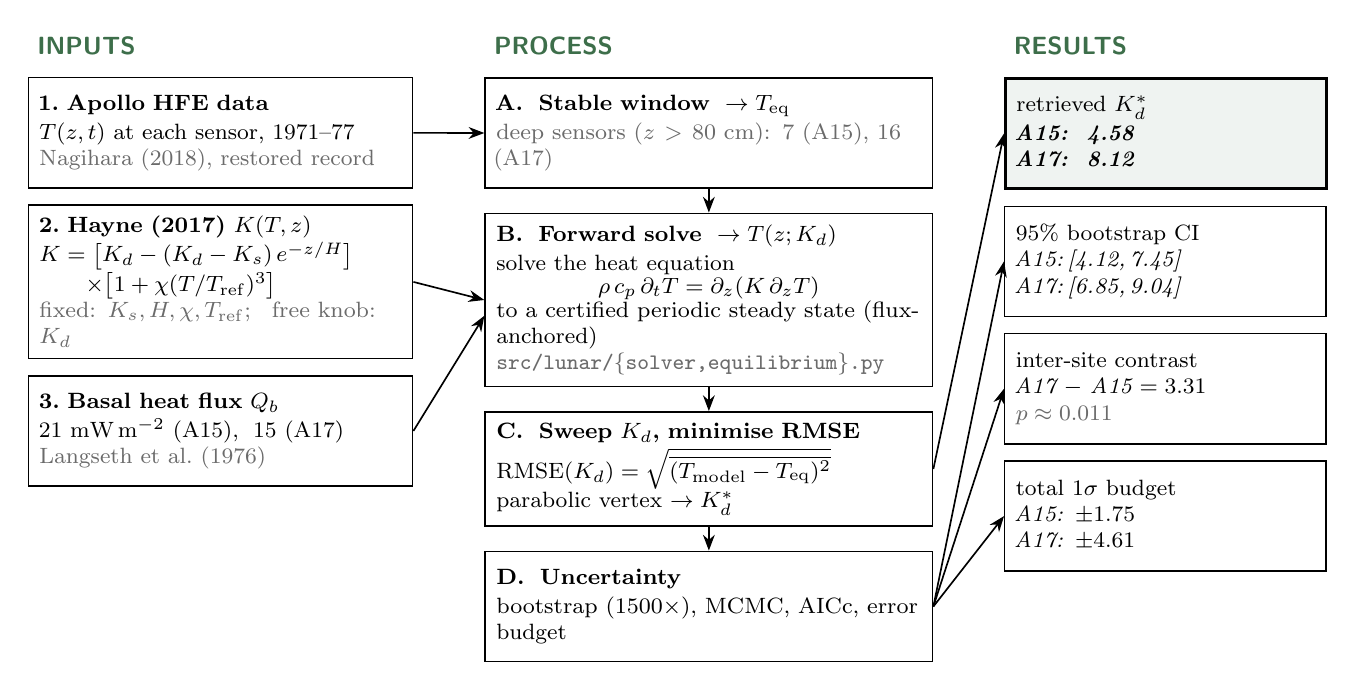
\begin{tikzpicture}[
  font=\footnotesize,
  every node/.style={align=left},
  inb/.style={rectangle, draw=black, line width=0.5pt, fill=white,
              inner sep=4pt, text width=46mm, minimum height=14mm,
              anchor=north west},
  prb/.style={rectangle, draw=black, line width=0.6pt, fill=white,
              inner sep=4pt, text width=54mm, minimum height=14mm,
              anchor=north west},
  rsb/.style={rectangle, draw=black, line width=0.5pt, fill=white,
              inner sep=4pt, text width=38mm, minimum height=14mm,
              anchor=north west},
  hl/.style={rsb, line width=0.9pt, fill=forest!8},
  col/.style={font=\sffamily\bfseries\small\color{forest}, anchor=west},
  arr/.style={-{Stealth[length=2mm]}, line width=0.6pt}
]
% --- column anchor x-coordinates (all in cm) ---
% inputs:  x=0..4.6        (4.6 wide)
% process: x=5.8..11.2      (5.4 wide, +1.2 gap)
% results: x=12.4..16.2     (3.8 wide, +1.2 gap)
\node[col]                  at (0,    0) (HI) {INPUTS};
\node[col]                  at (5.8,  0) (HP) {PROCESS};
\node[col]                  at (12.4, 0) (HR) {RESULTS};

% --- INPUTS column ---
\node[inb] at (0,-0.4)  (i1) {%
  \textbf{1.\;Apollo HFE data}\\[1pt]
  $T(z,t)$ at each sensor, 1971--77\\
  {\color{dim}Nagihara (2018), restored record}};
\node[inb, below=2mm of i1.south west, anchor=north west] (i2) {%
  \textbf{2.\;Hayne (2017) $K(T,z)$}\\[1pt]
  $K=\bigl[K_d-(K_d-K_s)\,e^{-z/H}\bigr]$\\
  \hphantom{$K=$}$\times\bigl[1+\chi(T/T_{\rm ref})^3\bigr]$\\
  {\color{dim}fixed: $K_s,H,\chi,T_{\rm ref}$;\;\; free knob: $K_d$}};
\node[inb, below=2mm of i2.south west, anchor=north west] (i3) {%
  \textbf{3.\;Basal heat flux $Q_b$}\\[1pt]
  $21$ mW\,m$^{-2}$ (A15),\; $15$ (A17)\\
  {\color{dim}Langseth et al.\ (1976)}};

% --- PROCESS column ---
\node[prb] at (5.8,-0.4)  (pA) {%
  \textbf{A.\; Stable window\; $\to T_{\rm eq}$}\\[1pt]
  {\color{dim}deep sensors ($z>80$ cm): 7 (A15), 16 (A17)}};
\node[prb, below=3mm of pA.south west, anchor=north west,
      minimum height=22mm] (pB) {%
  \textbf{B.\; Forward solve\; $\to T(z;K_d)$}\\[1pt]
  solve the heat equation\\[-1pt]
  \hfill$\rho\,c_p\,\partial_t T=\partial_z(K\,\partial_z T)$\hfill\null\\[-1pt]
  to a certified periodic steady state (flux-anchored)\\
  {\color{dim}\texttt{src/lunar/\{solver,equilibrium\}.py}}};
\node[prb, below=3mm of pB.south west, anchor=north west] (pC) {%
  \textbf{C.\; Sweep $K_d$, minimise RMSE}\\[1pt]
  $\mathrm{RMSE}(K_d)=\sqrt{\overline{(T_{\rm model}-T_{\rm eq})^2}}$\\
  parabolic vertex $\to K_d^{*}$};
\node[prb, below=3mm of pC.south west, anchor=north west] (pD) {%
  \textbf{D.\; Uncertainty}\\[1pt]
  bootstrap (1500$\times$), MCMC, AICc, error budget};

% --- RESULTS column ---
\node[hl]  at (12.4,-0.4)  (r1) {%
  retrieved $K_d^{*}$\\[1pt]
  \textbf{\itshape A15:\; 4.58}\\
  \textbf{\itshape A17:\; 8.12}};
\node[rsb, below=2mm of r1.south west, anchor=north west] (r2) {%
  95\% bootstrap CI\\
  \itshape A15:\,[4.12,\,7.45]\\
  \itshape A17:\,[6.85,\,9.04]};
\node[rsb, below=2mm of r2.south west, anchor=north west] (r3) {%
  inter-site contrast\\
  \itshape A17 $-$ A15 $= 3.31$\\
  {\color{dim}$p\approx 0.011$}};
\node[rsb, below=2mm of r3.south west, anchor=north west] (r4) {%
  total $1\sigma$ budget\\
  \itshape A15: $\pm 1.75$\\
  \itshape A17: $\pm 4.61$};

% --- arrows: inputs to process ---
\draw[arr] (i1.east) -- (pA.west);
\draw[arr] (i2.east) -- (pB.west);
\draw[arr] (i3.east) -- ($(pB.west)+(0,-2mm)$);

% --- arrows: process flow downward ---
\draw[arr] (pA.south) -- (pB.north);
\draw[arr] (pB.south) -- (pC.north);
\draw[arr] (pC.south) -- (pD.north);

% --- arrows: process to results ---
\draw[arr] (pC.east) -- (r1.west);
\draw[arr] (pD.east) -- (r2.west);
\draw[arr] (pD.east) -- (r3.west);
\draw[arr] (pD.east) -- (r4.west);
\end{tikzpicture}
 inside a
% figure environment that supplies its own \caption and \label.
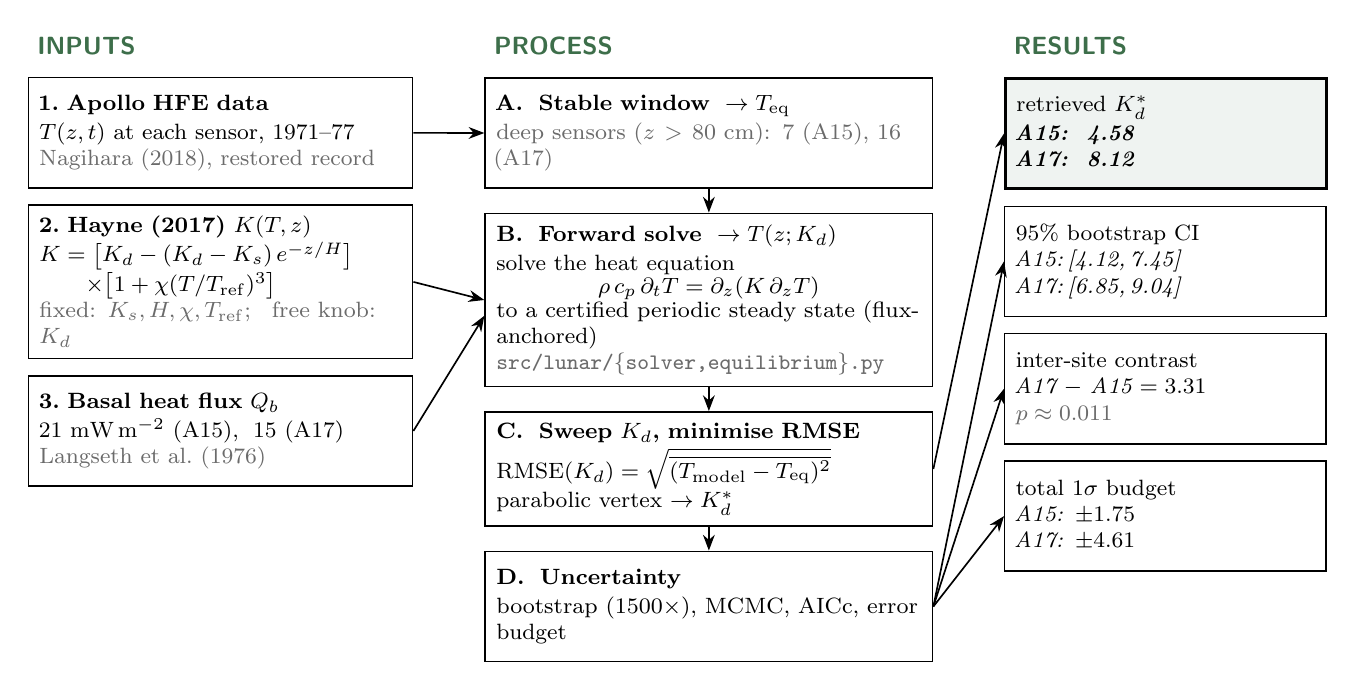
\begin{tikzpicture}[
  font=\footnotesize,
  every node/.style={align=left},
  inb/.style={rectangle, draw=black, line width=0.5pt, fill=white,
              inner sep=4pt, text width=46mm, minimum height=14mm,
              anchor=north west},
  prb/.style={rectangle, draw=black, line width=0.6pt, fill=white,
              inner sep=4pt, text width=54mm, minimum height=14mm,
              anchor=north west},
  rsb/.style={rectangle, draw=black, line width=0.5pt, fill=white,
              inner sep=4pt, text width=38mm, minimum height=14mm,
              anchor=north west},
  hl/.style={rsb, line width=0.9pt, fill=forest!8},
  col/.style={font=\sffamily\bfseries\small\color{forest}, anchor=west},
  arr/.style={-{Stealth[length=2mm]}, line width=0.6pt}
]
% --- column anchor x-coordinates (all in cm) ---
% inputs:  x=0..4.6        (4.6 wide)
% process: x=5.8..11.2      (5.4 wide, +1.2 gap)
% results: x=12.4..16.2     (3.8 wide, +1.2 gap)
\node[col]                  at (0,    0) (HI) {INPUTS};
\node[col]                  at (5.8,  0) (HP) {PROCESS};
\node[col]                  at (12.4, 0) (HR) {RESULTS};

% --- INPUTS column ---
\node[inb] at (0,-0.4)  (i1) {%
  \textbf{1.\;Apollo HFE data}\\[1pt]
  $T(z,t)$ at each sensor, 1971--77\\
  {\color{dim}Nagihara (2018), restored record}};
\node[inb, below=2mm of i1.south west, anchor=north west] (i2) {%
  \textbf{2.\;Hayne (2017) $K(T,z)$}\\[1pt]
  $K=\bigl[K_d-(K_d-K_s)\,e^{-z/H}\bigr]$\\
  \hphantom{$K=$}$\times\bigl[1+\chi(T/T_{\rm ref})^3\bigr]$\\
  {\color{dim}fixed: $K_s,H,\chi,T_{\rm ref}$;\;\; free knob: $K_d$}};
\node[inb, below=2mm of i2.south west, anchor=north west] (i3) {%
  \textbf{3.\;Basal heat flux $Q_b$}\\[1pt]
  $21$ mW\,m$^{-2}$ (A15),\; $15$ (A17)\\
  {\color{dim}Langseth et al.\ (1976)}};

% --- PROCESS column ---
\node[prb] at (5.8,-0.4)  (pA) {%
  \textbf{A.\; Stable window\; $\to T_{\rm eq}$}\\[1pt]
  {\color{dim}deep sensors ($z>80$ cm): 7 (A15), 16 (A17)}};
\node[prb, below=3mm of pA.south west, anchor=north west,
      minimum height=22mm] (pB) {%
  \textbf{B.\; Forward solve\; $\to T(z;K_d)$}\\[1pt]
  solve the heat equation\\[-1pt]
  \hfill$\rho\,c_p\,\partial_t T=\partial_z(K\,\partial_z T)$\hfill\null\\[-1pt]
  to a certified periodic steady state (flux-anchored)\\
  {\color{dim}\texttt{src/lunar/\{solver,equilibrium\}.py}}};
\node[prb, below=3mm of pB.south west, anchor=north west] (pC) {%
  \textbf{C.\; Sweep $K_d$, minimise RMSE}\\[1pt]
  $\mathrm{RMSE}(K_d)=\sqrt{\overline{(T_{\rm model}-T_{\rm eq})^2}}$\\
  parabolic vertex $\to K_d^{*}$};
\node[prb, below=3mm of pC.south west, anchor=north west] (pD) {%
  \textbf{D.\; Uncertainty}\\[1pt]
  bootstrap (1500$\times$), MCMC, AICc, error budget};

% --- RESULTS column ---
\node[hl]  at (12.4,-0.4)  (r1) {%
  retrieved $K_d^{*}$\\[1pt]
  \textbf{\itshape A15:\; 4.58}\\
  \textbf{\itshape A17:\; 8.12}};
\node[rsb, below=2mm of r1.south west, anchor=north west] (r2) {%
  95\% bootstrap CI\\
  \itshape A15:\,[4.12,\,7.45]\\
  \itshape A17:\,[6.85,\,9.04]};
\node[rsb, below=2mm of r2.south west, anchor=north west] (r3) {%
  inter-site contrast\\
  \itshape A17 $-$ A15 $= 3.31$\\
  {\color{dim}$p\approx 0.011$}};
\node[rsb, below=2mm of r3.south west, anchor=north west] (r4) {%
  total $1\sigma$ budget\\
  \itshape A15: $\pm 1.75$\\
  \itshape A17: $\pm 4.61$};

% --- arrows: inputs to process ---
\draw[arr] (i1.east) -- (pA.west);
\draw[arr] (i2.east) -- (pB.west);
\draw[arr] (i3.east) -- ($(pB.west)+(0,-2mm)$);

% --- arrows: process flow downward ---
\draw[arr] (pA.south) -- (pB.north);
\draw[arr] (pB.south) -- (pC.north);
\draw[arr] (pC.south) -- (pD.north);

% --- arrows: process to results ---
\draw[arr] (pC.east) -- (r1.west);
\draw[arr] (pD.east) -- (r2.west);
\draw[arr] (pD.east) -- (r3.west);
\draw[arr] (pD.east) -- (r4.west);
\end{tikzpicture}
 inside a
% figure environment that supplies its own \caption and \label.
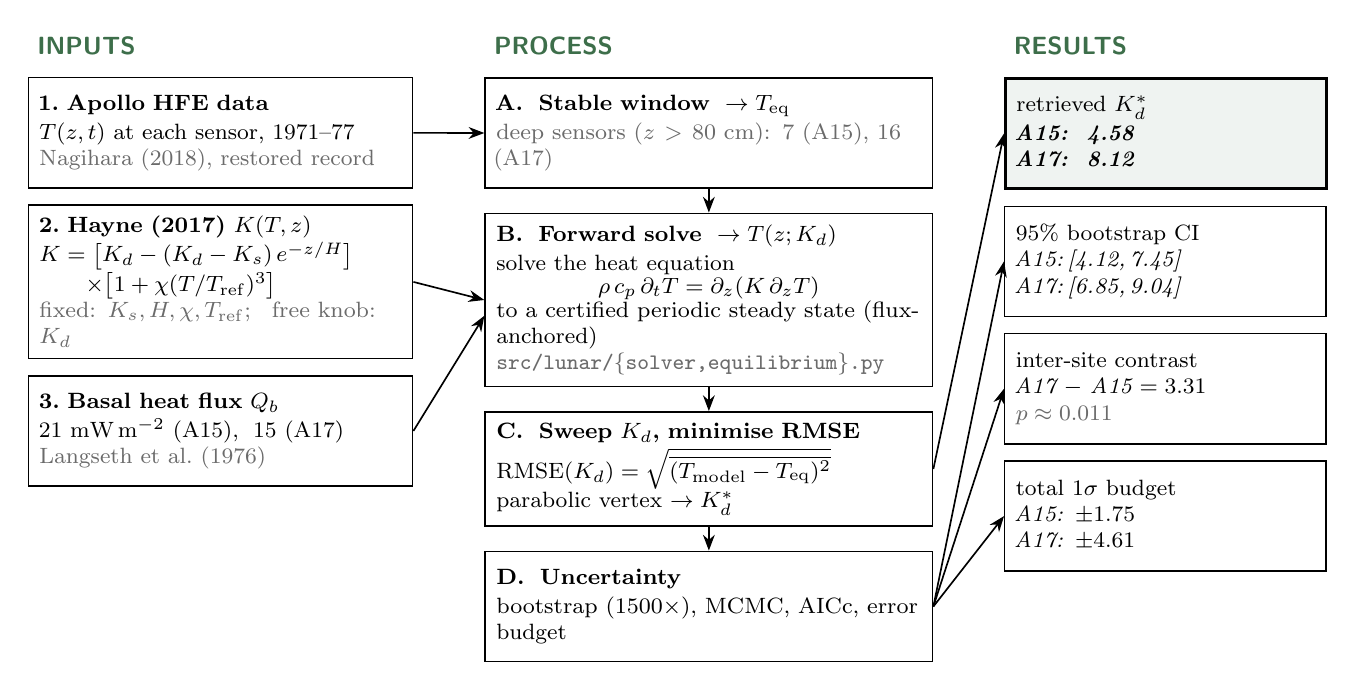
\begin{tikzpicture}[
  font=\footnotesize,
  every node/.style={align=left},
  inb/.style={rectangle, draw=black, line width=0.5pt, fill=white,
              inner sep=4pt, text width=46mm, minimum height=14mm,
              anchor=north west},
  prb/.style={rectangle, draw=black, line width=0.6pt, fill=white,
              inner sep=4pt, text width=54mm, minimum height=14mm,
              anchor=north west},
  rsb/.style={rectangle, draw=black, line width=0.5pt, fill=white,
              inner sep=4pt, text width=38mm, minimum height=14mm,
              anchor=north west},
  hl/.style={rsb, line width=0.9pt, fill=forest!8},
  col/.style={font=\sffamily\bfseries\small\color{forest}, anchor=west},
  arr/.style={-{Stealth[length=2mm]}, line width=0.6pt}
]
% --- column anchor x-coordinates (all in cm) ---
% inputs:  x=0..4.6        (4.6 wide)
% process: x=5.8..11.2      (5.4 wide, +1.2 gap)
% results: x=12.4..16.2     (3.8 wide, +1.2 gap)
\node[col]                  at (0,    0) (HI) {INPUTS};
\node[col]                  at (5.8,  0) (HP) {PROCESS};
\node[col]                  at (12.4, 0) (HR) {RESULTS};

% --- INPUTS column ---
\node[inb] at (0,-0.4)  (i1) {%
  \textbf{1.\;Apollo HFE data}\\[1pt]
  $T(z,t)$ at each sensor, 1971--77\\
  {\color{dim}Nagihara (2018), restored record}};
\node[inb, below=2mm of i1.south west, anchor=north west] (i2) {%
  \textbf{2.\;Hayne (2017) $K(T,z)$}\\[1pt]
  $K=\bigl[K_d-(K_d-K_s)\,e^{-z/H}\bigr]$\\
  \hphantom{$K=$}$\times\bigl[1+\chi(T/T_{\rm ref})^3\bigr]$\\
  {\color{dim}fixed: $K_s,H,\chi,T_{\rm ref}$;\;\; free knob: $K_d$}};
\node[inb, below=2mm of i2.south west, anchor=north west] (i3) {%
  \textbf{3.\;Basal heat flux $Q_b$}\\[1pt]
  $21$ mW\,m$^{-2}$ (A15),\; $15$ (A17)\\
  {\color{dim}Langseth et al.\ (1976)}};

% --- PROCESS column ---
\node[prb] at (5.8,-0.4)  (pA) {%
  \textbf{A.\; Stable window\; $\to T_{\rm eq}$}\\[1pt]
  {\color{dim}deep sensors ($z>80$ cm): 7 (A15), 16 (A17)}};
\node[prb, below=3mm of pA.south west, anchor=north west,
      minimum height=22mm] (pB) {%
  \textbf{B.\; Forward solve\; $\to T(z;K_d)$}\\[1pt]
  solve the heat equation\\[-1pt]
  \hfill$\rho\,c_p\,\partial_t T=\partial_z(K\,\partial_z T)$\hfill\null\\[-1pt]
  to a certified periodic steady state (flux-anchored)\\
  {\color{dim}\texttt{src/lunar/\{solver,equilibrium\}.py}}};
\node[prb, below=3mm of pB.south west, anchor=north west] (pC) {%
  \textbf{C.\; Sweep $K_d$, minimise RMSE}\\[1pt]
  $\mathrm{RMSE}(K_d)=\sqrt{\overline{(T_{\rm model}-T_{\rm eq})^2}}$\\
  parabolic vertex $\to K_d^{*}$};
\node[prb, below=3mm of pC.south west, anchor=north west] (pD) {%
  \textbf{D.\; Uncertainty}\\[1pt]
  bootstrap (1500$\times$), MCMC, AICc, error budget};

% --- RESULTS column ---
\node[hl]  at (12.4,-0.4)  (r1) {%
  retrieved $K_d^{*}$\\[1pt]
  \textbf{\itshape A15:\; 4.58}\\
  \textbf{\itshape A17:\; 8.12}};
\node[rsb, below=2mm of r1.south west, anchor=north west] (r2) {%
  95\% bootstrap CI\\
  \itshape A15:\,[4.12,\,7.45]\\
  \itshape A17:\,[6.85,\,9.04]};
\node[rsb, below=2mm of r2.south west, anchor=north west] (r3) {%
  inter-site contrast\\
  \itshape A17 $-$ A15 $= 3.31$\\
  {\color{dim}$p\approx 0.011$}};
\node[rsb, below=2mm of r3.south west, anchor=north west] (r4) {%
  total $1\sigma$ budget\\
  \itshape A15: $\pm 1.75$\\
  \itshape A17: $\pm 4.61$};

% --- arrows: inputs to process ---
\draw[arr] (i1.east) -- (pA.west);
\draw[arr] (i2.east) -- (pB.west);
\draw[arr] (i3.east) -- ($(pB.west)+(0,-2mm)$);

% --- arrows: process flow downward ---
\draw[arr] (pA.south) -- (pB.north);
\draw[arr] (pB.south) -- (pC.north);
\draw[arr] (pC.south) -- (pD.north);

% --- arrows: process to results ---
\draw[arr] (pC.east) -- (r1.west);
\draw[arr] (pD.east) -- (r2.west);
\draw[arr] (pD.east) -- (r3.west);
\draw[arr] (pD.east) -- (r4.west);
\end{tikzpicture}

\caption{The retrieval pipeline. Three inputs (Apollo data; the Hayne
conductivity model with one free knob $K_d$; the published basal flux $Q_b$)
feed four processes (extract equilibrium temperatures; solve the heat equation
forward to a certified steady state; sweep $K_d$ to minimise the deep-sensor
RMSE; quantify uncertainty). The boxed heat equation is the physical core; the
rest is bookkeeping around it.}
\label{fig:pipeline}
\end{figure}

Figure~\ref{fig:pipeline} shows the \emph{processes}; Figure~\ref{fig:eqnflow}
shows the \emph{equations} --- every formula in the study laid out in the order
it is used, with arrows tracing what produces which variable and feeds the next.
If you ever lose the thread of ``where does this expression come from and what
does it feed?'', that is the map.

\begin{figure}[p]\centering
% Fig 1.5 — equation flow from inputs to the final K_d*.
% This file contains only the tikzpicture body.  Iterate via:
%   pdflatex eqnflow_standalone.tex
% In the book it is consumed via % Fig 1.5 — equation flow from inputs to the final K_d*.
% This file contains only the tikzpicture body.  Iterate via:
%   pdflatex eqnflow_standalone.tex
% In the book it is consumed via % Fig 1.5 — equation flow from inputs to the final K_d*.
% This file contains only the tikzpicture body.  Iterate via:
%   pdflatex eqnflow_standalone.tex
% In the book it is consumed via \input{figures-tikz/eqnflow} inside a
% figure environment that supplies its own \caption and \label.
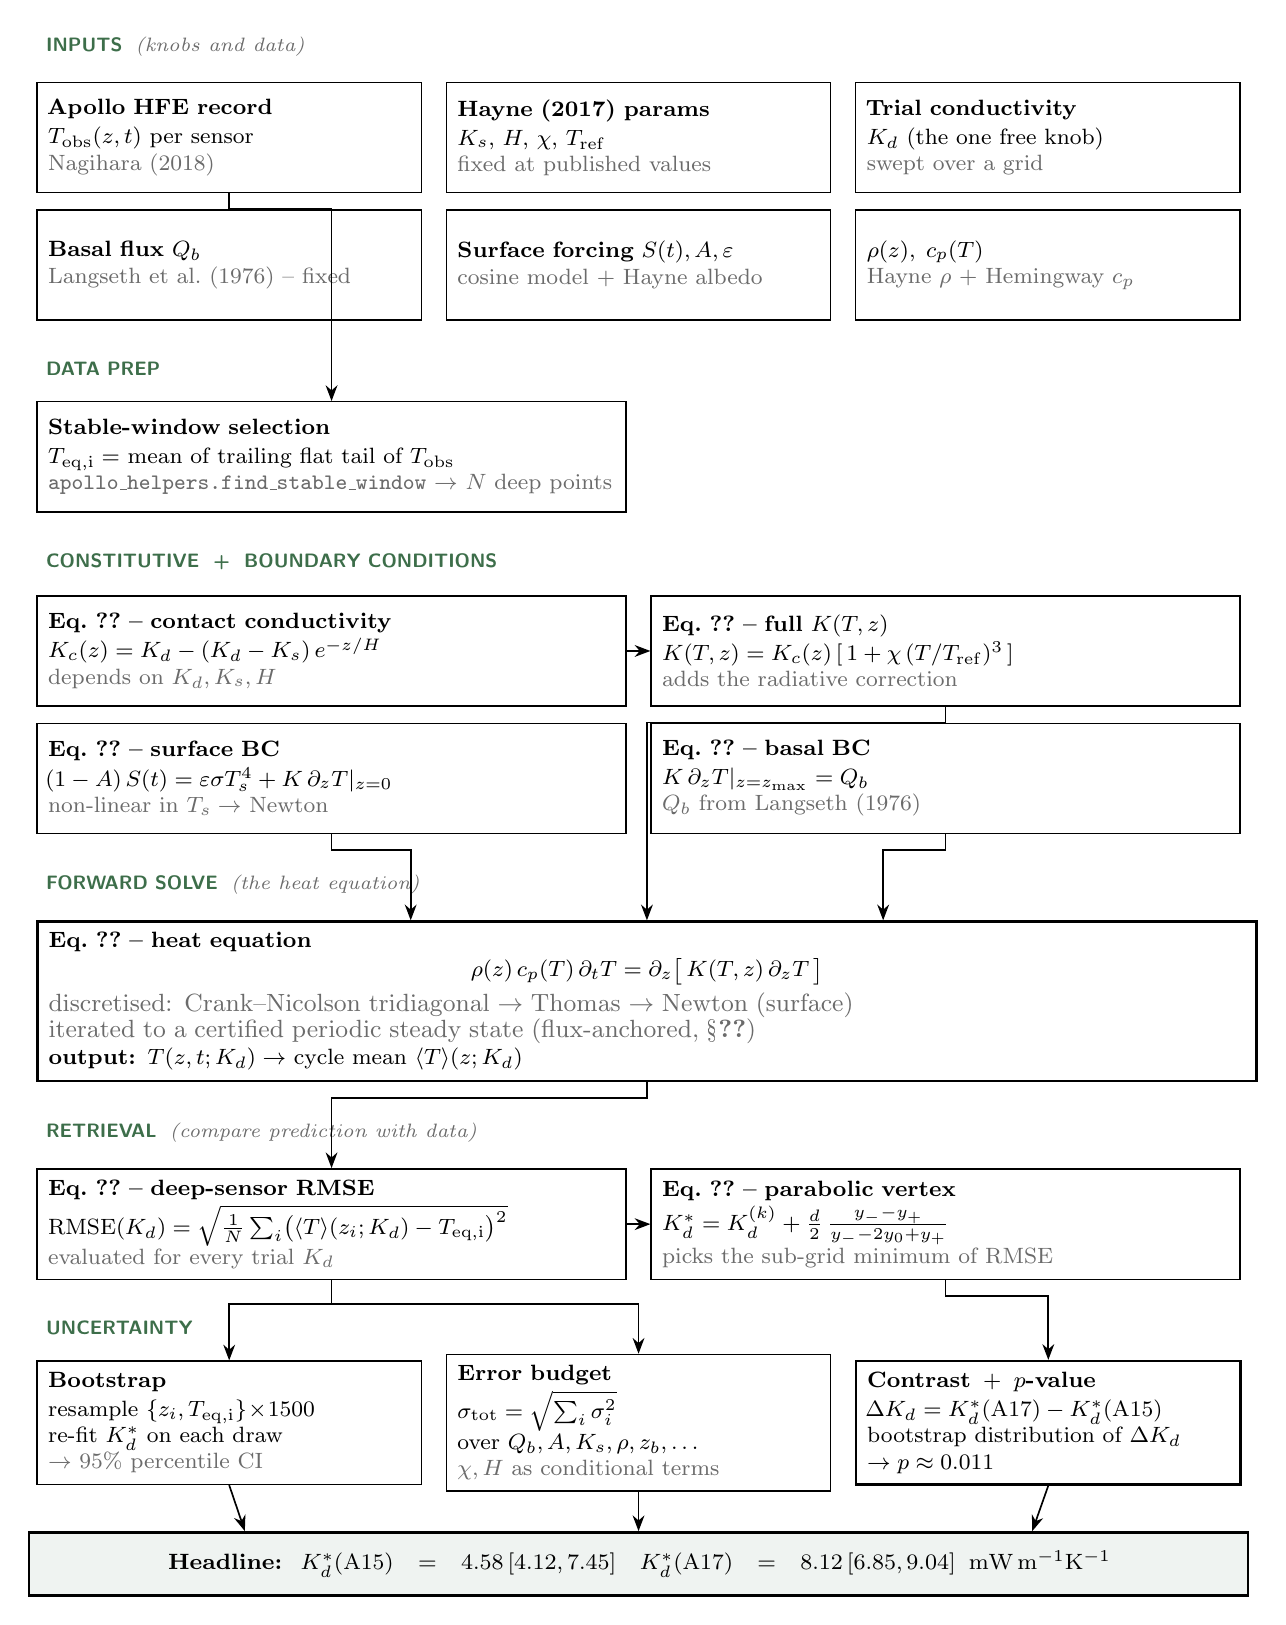
\begin{tikzpicture}[
  font=\footnotesize,
  every node/.style={align=left},
  box/.style={rectangle, draw=black, line width=0.5pt, inner sep=4pt,
              text width=46mm, minimum height=14mm, fill=white},
  wide/.style={text width=152mm},
  half/.style={text width=72mm},
  bandlabel/.style={font=\sffamily\bfseries\scriptsize\color{forest},
                    anchor=west},
  arr/.style={-{Stealth[length=2mm]}, line width=0.6pt}
]
% ---------- LEVEL 1: INPUTS ----------
\node[bandlabel] (L1) at (-78mm, 0) {INPUTS \;\textnormal{\color{dim}\itshape (knobs and data)}};
\node[box, below=2mm of L1.south west, anchor=north west] (in1)
  {\textbf{Apollo HFE record}\\[1pt]
   $T_{\rm obs}(z,t)$ per sensor\\
   {\color{dim}Nagihara (2018)}};
\node[box, right=3mm of in1] (in2)
  {\textbf{Hayne (2017) params}\\[1pt]
   $K_s,\,H,\,\chi,\,T_{\rm ref}$\\
   {\color{dim}fixed at published values}};
\node[box, right=3mm of in2] (in3)
  {\textbf{Trial conductivity}\\[1pt]
   $K_d$ (the one free knob)\\
   {\color{dim}swept over a grid}};
\node[box, below=2mm of in1] (in4)
  {\textbf{Basal flux $Q_b$}\\
   {\color{dim}Langseth et al.\ (1976) -- fixed}};
\node[box, below=2mm of in2] (in5)
  {\textbf{Surface forcing $S(t),A,\varepsilon$}\\
   {\color{dim}cosine model + Hayne albedo}};
\node[box, below=2mm of in3] (in6)
  {\textbf{$\rho(z),\;c_p(T)$}\\
   {\color{dim}Hayne $\rho$ + Hemingway $c_p$}};

% ---------- LEVEL 2: DATA PREP ----------
\node[bandlabel, below=4mm of in4.south west, anchor=north west] (L2)
  {DATA PREP};
\node[box, half, below=2mm of L2.south west, anchor=north west] (dp)
  {\textbf{Stable-window selection}\\[1pt]
   $T_{\rm eq,i}=$ mean of trailing flat tail of $T_{\rm obs}$\\
   {\color{dim}\texttt{apollo\_helpers.find\_stable\_window} $\to$ $N$ deep points}};
\draw[arr] (in1.south) -- ++(0,-2mm) -| (dp.north);

% ---------- LEVEL 3: CONSTITUTIVE + BC ----------
\node[bandlabel, below=4mm of dp.south west, anchor=north west] (L3)
  {CONSTITUTIVE\ \ +\ \ BOUNDARY CONDITIONS};
\node[box, half, below=2mm of L3.south west, anchor=north west] (eqKc)
  {\textbf{Eq.~\ref{eq:Kc} -- contact conductivity}\\[1pt]
   $K_c(z)=K_d-(K_d-K_s)\,e^{-z/H}$\\
   {\color{dim}depends on $K_d,K_s,H$}};
\node[box, half, right=3mm of eqKc] (eqK)
  {\textbf{Eq.~\ref{eq:Khayne} -- full $K(T,z)$}\\[1pt]
   $K(T,z)=K_c(z)\,[\,1+\chi\,(T/T_{\rm ref})^3\,]$\\
   {\color{dim}adds the radiative correction}};
\node[box, half, below=2mm of eqKc] (bcS)
  {\textbf{Eq.~\ref{eq:surfbc} -- surface BC}\\[1pt]
   $(1-A)\,S(t)=\varepsilon\sigma T_s^4+K\,\partial_z T|_{z=0}$\\
   {\color{dim}non-linear in $T_s\to$ Newton}};
\node[box, half, right=3mm of bcS] (bcB)
  {\textbf{Eq.~\ref{eq:bottombc} -- basal BC}\\[1pt]
   $K\,\partial_z T|_{z=z_{\max}}=Q_b$\\
   {\color{dim}$Q_b$ from Langseth (1976)}};
\draw[arr] (eqKc.east) -- (eqK.west);

% ---------- LEVEL 4: PDE ----------
\node[bandlabel, below=4mm of bcS.south west, anchor=north west] (L4)
  {FORWARD SOLVE \;\textnormal{\color{dim}\itshape (the heat equation)}};
\node[box, wide, below=2mm of L4.south west, anchor=north west,
      minimum height=20mm, line width=0.8pt] (pde) {%
  \textbf{Eq.~\ref{eq:heat} -- heat equation}\\[1pt]
  \hfill$\displaystyle \rho(z)\,c_p(T)\,\partial_t T=\partial_z\bigl[\,K(T,z)\,\partial_z T\,\bigr]$\hfill\null\\[2pt]
  {\color{dim}\small discretised: Crank--Nicolson tridiagonal $\to$ Thomas $\to$ Newton (surface)}\\
  {\color{dim}\small iterated to a certified periodic steady state (flux-anchored, \S\ref{sec:cert})}\\
  \textbf{output:} $T(z,t;K_d)\to$ cycle mean $\langle T\rangle(z;K_d)$};
\draw[arr] (eqK.south) -- ++(0,-2mm) -| (pde.north);
\draw[arr] (bcS.south) -- ++(0,-2mm) -| ($(pde.north)+(-30mm,0)$);
\draw[arr] (bcB.south) -- ++(0,-2mm) -| ($(pde.north)+(30mm,0)$);

% ---------- LEVEL 5: RETRIEVAL ----------
\node[bandlabel, below=4mm of pde.south west, anchor=north west] (L5)
  {RETRIEVAL \;\textnormal{\color{dim}\itshape (compare prediction with data)}};
\node[box, half, below=2mm of L5.south west, anchor=north west] (rmse)
  {\textbf{Eq.~\ref{eq:rmse} -- deep-sensor RMSE}\\[1pt]
   $\mathrm{RMSE}(K_d)=\sqrt{\tfrac{1}{N}\sum_i\bigl(\langle T\rangle(z_i;K_d)-T_{\rm eq,i}\bigr)^2}$\\
   {\color{dim}evaluated for every trial $K_d$}};
\node[box, half, right=3mm of rmse] (vertex)
  {\textbf{Eq.~\ref{eq:vertex} -- parabolic vertex}\\[1pt]
   $K_d^{*}=K_d^{(k)}+\tfrac{d}{2}\,\tfrac{y_--y_+}{y_--2y_0+y_+}$\\
   {\color{dim}picks the sub-grid minimum of RMSE}};
\draw[arr] (pde.south) -- ++(0,-2mm) -| (rmse.north);
\draw[arr] (rmse.east) -- (vertex.west);

% ---------- LEVEL 6: UNCERTAINTY ----------
\node[bandlabel, below=4mm of rmse.south west, anchor=north west] (L6)
  {UNCERTAINTY};
\node[box, below=2mm of L6.south west, anchor=north west] (boot)
  {\textbf{Bootstrap}\\[1pt]
   resample $\{z_i,T_{\rm eq,i}\}\!\times\!1500$\\
   re-fit $K_d^{*}$ on each draw\\
   {\color{dim}$\to$ 95\% percentile CI}};
\node[box, right=3mm of boot] (budg)
  {\textbf{Error budget}\\[1pt]
   $\sigma_{\rm tot}=\sqrt{\sum_i\sigma_i^2}$\\
   over $Q_b,A,K_s,\rho,z_b,\ldots$\\
   {\color{dim}$\chi,H$ as conditional terms}};
\node[box, right=3mm of budg, line width=0.8pt] (contr)
  {\textbf{Contrast \,$+$\, $p$-value}\\[1pt]
   $\Delta K_d=K_d^{*}({\rm A17})-K_d^{*}({\rm A15})$\\
   bootstrap distribution of $\Delta K_d$\\
   $\to p\approx 0.011$};
\draw[arr] (vertex.south) -- ++(0,-2mm) -| (contr.north);
\draw[arr] (rmse.south) -- ++(0,-3mm) -| (boot.north);
\draw[arr] (rmse.south) -- ++(0,-3mm) -| (budg.north);

% ---------- RESULT STRIP ----------
\node[draw=black, line width=1pt, fill=forest!8,
      text width=152mm, minimum height=8mm,
      below=5mm of budg.south, anchor=north,
      align=center, inner sep=4pt] (out)
  {\textbf{Headline:}\;
   $K_d^{*}({\rm A15})=4.58\,[4.12,7.45]$\quad
   $K_d^{*}({\rm A17})=8.12\,[6.85,9.04]$\;\;mW\,m$^{-1}$K$^{-1}$};
\draw[arr] (boot.south)  -- ($(out.north)+(-50mm,0)$);
\draw[arr] (budg.south)  -- (out.north);
\draw[arr] (contr.south) -- ($(out.north)+(50mm,0)$);
\end{tikzpicture}
 inside a
% figure environment that supplies its own \caption and \label.
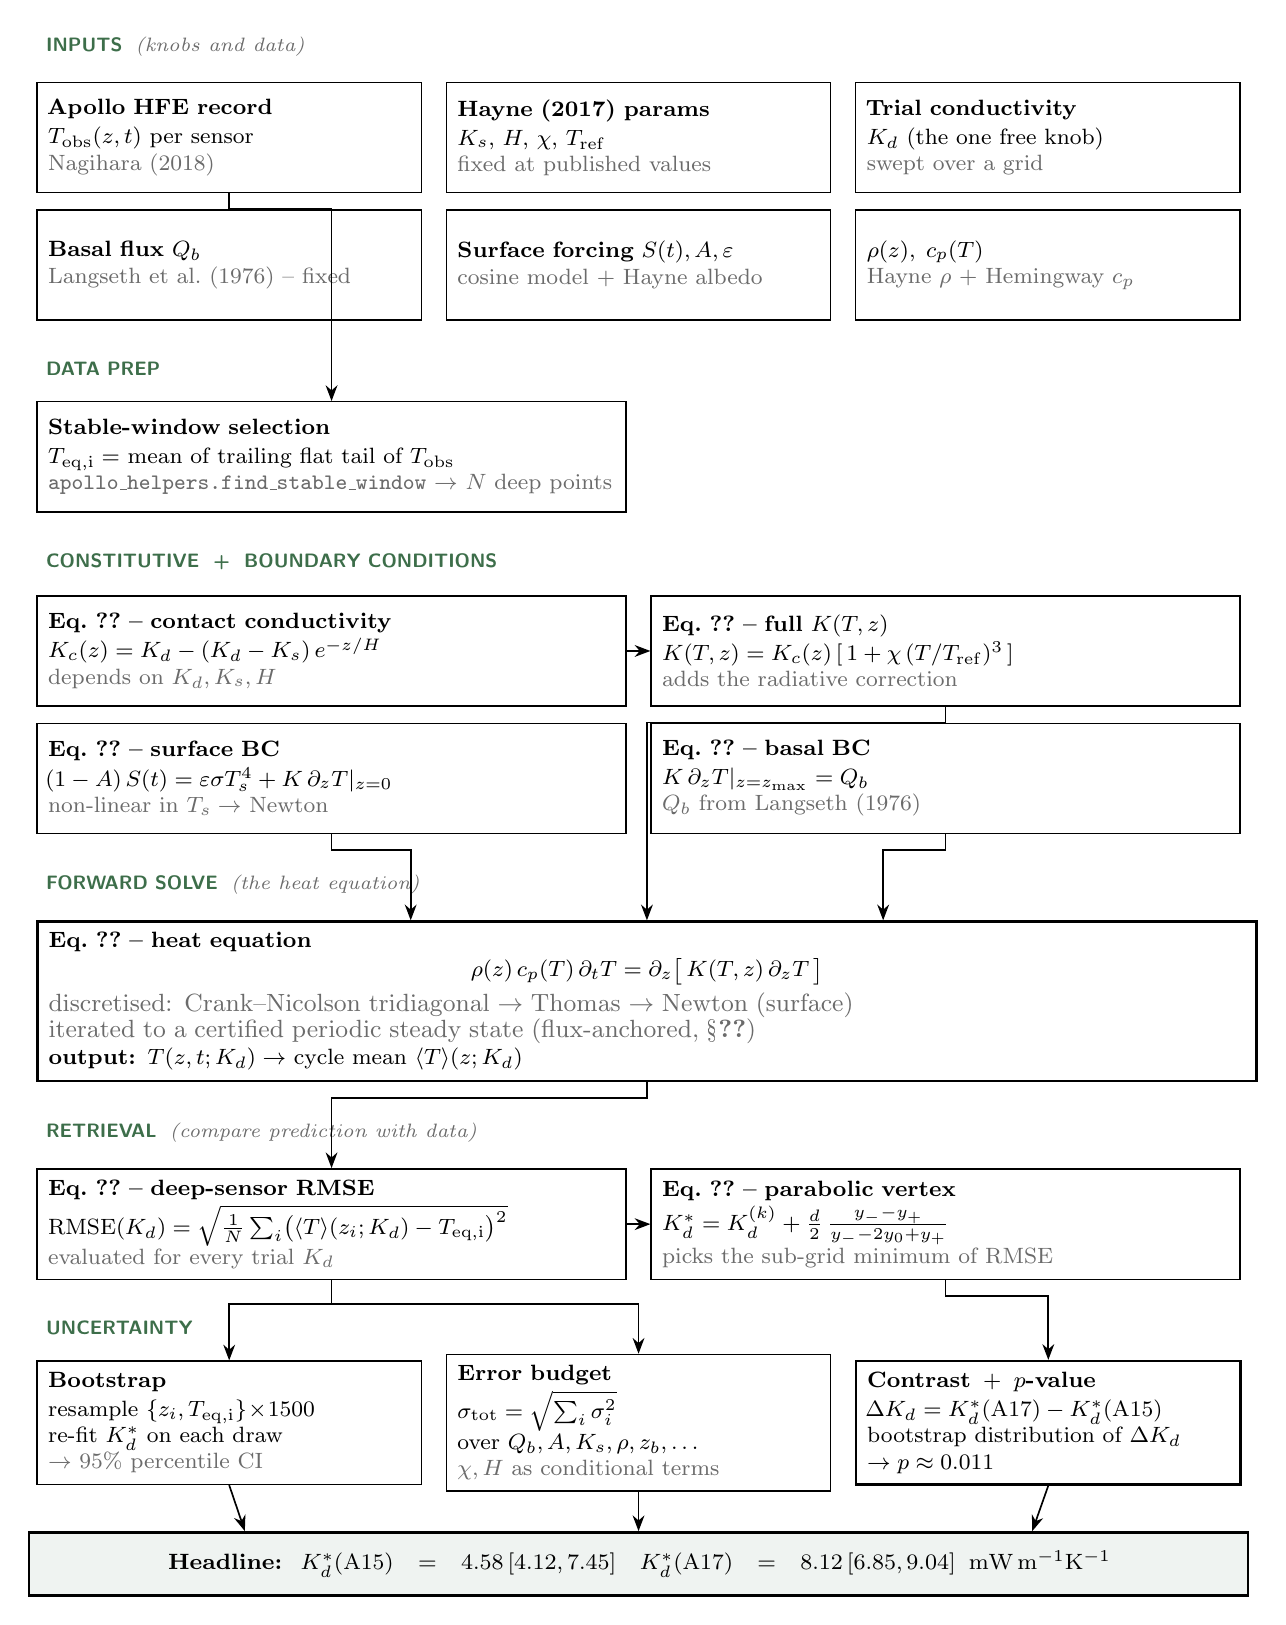
\begin{tikzpicture}[
  font=\footnotesize,
  every node/.style={align=left},
  box/.style={rectangle, draw=black, line width=0.5pt, inner sep=4pt,
              text width=46mm, minimum height=14mm, fill=white},
  wide/.style={text width=152mm},
  half/.style={text width=72mm},
  bandlabel/.style={font=\sffamily\bfseries\scriptsize\color{forest},
                    anchor=west},
  arr/.style={-{Stealth[length=2mm]}, line width=0.6pt}
]
% ---------- LEVEL 1: INPUTS ----------
\node[bandlabel] (L1) at (-78mm, 0) {INPUTS \;\textnormal{\color{dim}\itshape (knobs and data)}};
\node[box, below=2mm of L1.south west, anchor=north west] (in1)
  {\textbf{Apollo HFE record}\\[1pt]
   $T_{\rm obs}(z,t)$ per sensor\\
   {\color{dim}Nagihara (2018)}};
\node[box, right=3mm of in1] (in2)
  {\textbf{Hayne (2017) params}\\[1pt]
   $K_s,\,H,\,\chi,\,T_{\rm ref}$\\
   {\color{dim}fixed at published values}};
\node[box, right=3mm of in2] (in3)
  {\textbf{Trial conductivity}\\[1pt]
   $K_d$ (the one free knob)\\
   {\color{dim}swept over a grid}};
\node[box, below=2mm of in1] (in4)
  {\textbf{Basal flux $Q_b$}\\
   {\color{dim}Langseth et al.\ (1976) -- fixed}};
\node[box, below=2mm of in2] (in5)
  {\textbf{Surface forcing $S(t),A,\varepsilon$}\\
   {\color{dim}cosine model + Hayne albedo}};
\node[box, below=2mm of in3] (in6)
  {\textbf{$\rho(z),\;c_p(T)$}\\
   {\color{dim}Hayne $\rho$ + Hemingway $c_p$}};

% ---------- LEVEL 2: DATA PREP ----------
\node[bandlabel, below=4mm of in4.south west, anchor=north west] (L2)
  {DATA PREP};
\node[box, half, below=2mm of L2.south west, anchor=north west] (dp)
  {\textbf{Stable-window selection}\\[1pt]
   $T_{\rm eq,i}=$ mean of trailing flat tail of $T_{\rm obs}$\\
   {\color{dim}\texttt{apollo\_helpers.find\_stable\_window} $\to$ $N$ deep points}};
\draw[arr] (in1.south) -- ++(0,-2mm) -| (dp.north);

% ---------- LEVEL 3: CONSTITUTIVE + BC ----------
\node[bandlabel, below=4mm of dp.south west, anchor=north west] (L3)
  {CONSTITUTIVE\ \ +\ \ BOUNDARY CONDITIONS};
\node[box, half, below=2mm of L3.south west, anchor=north west] (eqKc)
  {\textbf{Eq.~\ref{eq:Kc} -- contact conductivity}\\[1pt]
   $K_c(z)=K_d-(K_d-K_s)\,e^{-z/H}$\\
   {\color{dim}depends on $K_d,K_s,H$}};
\node[box, half, right=3mm of eqKc] (eqK)
  {\textbf{Eq.~\ref{eq:Khayne} -- full $K(T,z)$}\\[1pt]
   $K(T,z)=K_c(z)\,[\,1+\chi\,(T/T_{\rm ref})^3\,]$\\
   {\color{dim}adds the radiative correction}};
\node[box, half, below=2mm of eqKc] (bcS)
  {\textbf{Eq.~\ref{eq:surfbc} -- surface BC}\\[1pt]
   $(1-A)\,S(t)=\varepsilon\sigma T_s^4+K\,\partial_z T|_{z=0}$\\
   {\color{dim}non-linear in $T_s\to$ Newton}};
\node[box, half, right=3mm of bcS] (bcB)
  {\textbf{Eq.~\ref{eq:bottombc} -- basal BC}\\[1pt]
   $K\,\partial_z T|_{z=z_{\max}}=Q_b$\\
   {\color{dim}$Q_b$ from Langseth (1976)}};
\draw[arr] (eqKc.east) -- (eqK.west);

% ---------- LEVEL 4: PDE ----------
\node[bandlabel, below=4mm of bcS.south west, anchor=north west] (L4)
  {FORWARD SOLVE \;\textnormal{\color{dim}\itshape (the heat equation)}};
\node[box, wide, below=2mm of L4.south west, anchor=north west,
      minimum height=20mm, line width=0.8pt] (pde) {%
  \textbf{Eq.~\ref{eq:heat} -- heat equation}\\[1pt]
  \hfill$\displaystyle \rho(z)\,c_p(T)\,\partial_t T=\partial_z\bigl[\,K(T,z)\,\partial_z T\,\bigr]$\hfill\null\\[2pt]
  {\color{dim}\small discretised: Crank--Nicolson tridiagonal $\to$ Thomas $\to$ Newton (surface)}\\
  {\color{dim}\small iterated to a certified periodic steady state (flux-anchored, \S\ref{sec:cert})}\\
  \textbf{output:} $T(z,t;K_d)\to$ cycle mean $\langle T\rangle(z;K_d)$};
\draw[arr] (eqK.south) -- ++(0,-2mm) -| (pde.north);
\draw[arr] (bcS.south) -- ++(0,-2mm) -| ($(pde.north)+(-30mm,0)$);
\draw[arr] (bcB.south) -- ++(0,-2mm) -| ($(pde.north)+(30mm,0)$);

% ---------- LEVEL 5: RETRIEVAL ----------
\node[bandlabel, below=4mm of pde.south west, anchor=north west] (L5)
  {RETRIEVAL \;\textnormal{\color{dim}\itshape (compare prediction with data)}};
\node[box, half, below=2mm of L5.south west, anchor=north west] (rmse)
  {\textbf{Eq.~\ref{eq:rmse} -- deep-sensor RMSE}\\[1pt]
   $\mathrm{RMSE}(K_d)=\sqrt{\tfrac{1}{N}\sum_i\bigl(\langle T\rangle(z_i;K_d)-T_{\rm eq,i}\bigr)^2}$\\
   {\color{dim}evaluated for every trial $K_d$}};
\node[box, half, right=3mm of rmse] (vertex)
  {\textbf{Eq.~\ref{eq:vertex} -- parabolic vertex}\\[1pt]
   $K_d^{*}=K_d^{(k)}+\tfrac{d}{2}\,\tfrac{y_--y_+}{y_--2y_0+y_+}$\\
   {\color{dim}picks the sub-grid minimum of RMSE}};
\draw[arr] (pde.south) -- ++(0,-2mm) -| (rmse.north);
\draw[arr] (rmse.east) -- (vertex.west);

% ---------- LEVEL 6: UNCERTAINTY ----------
\node[bandlabel, below=4mm of rmse.south west, anchor=north west] (L6)
  {UNCERTAINTY};
\node[box, below=2mm of L6.south west, anchor=north west] (boot)
  {\textbf{Bootstrap}\\[1pt]
   resample $\{z_i,T_{\rm eq,i}\}\!\times\!1500$\\
   re-fit $K_d^{*}$ on each draw\\
   {\color{dim}$\to$ 95\% percentile CI}};
\node[box, right=3mm of boot] (budg)
  {\textbf{Error budget}\\[1pt]
   $\sigma_{\rm tot}=\sqrt{\sum_i\sigma_i^2}$\\
   over $Q_b,A,K_s,\rho,z_b,\ldots$\\
   {\color{dim}$\chi,H$ as conditional terms}};
\node[box, right=3mm of budg, line width=0.8pt] (contr)
  {\textbf{Contrast \,$+$\, $p$-value}\\[1pt]
   $\Delta K_d=K_d^{*}({\rm A17})-K_d^{*}({\rm A15})$\\
   bootstrap distribution of $\Delta K_d$\\
   $\to p\approx 0.011$};
\draw[arr] (vertex.south) -- ++(0,-2mm) -| (contr.north);
\draw[arr] (rmse.south) -- ++(0,-3mm) -| (boot.north);
\draw[arr] (rmse.south) -- ++(0,-3mm) -| (budg.north);

% ---------- RESULT STRIP ----------
\node[draw=black, line width=1pt, fill=forest!8,
      text width=152mm, minimum height=8mm,
      below=5mm of budg.south, anchor=north,
      align=center, inner sep=4pt] (out)
  {\textbf{Headline:}\;
   $K_d^{*}({\rm A15})=4.58\,[4.12,7.45]$\quad
   $K_d^{*}({\rm A17})=8.12\,[6.85,9.04]$\;\;mW\,m$^{-1}$K$^{-1}$};
\draw[arr] (boot.south)  -- ($(out.north)+(-50mm,0)$);
\draw[arr] (budg.south)  -- (out.north);
\draw[arr] (contr.south) -- ($(out.north)+(50mm,0)$);
\end{tikzpicture}
 inside a
% figure environment that supplies its own \caption and \label.
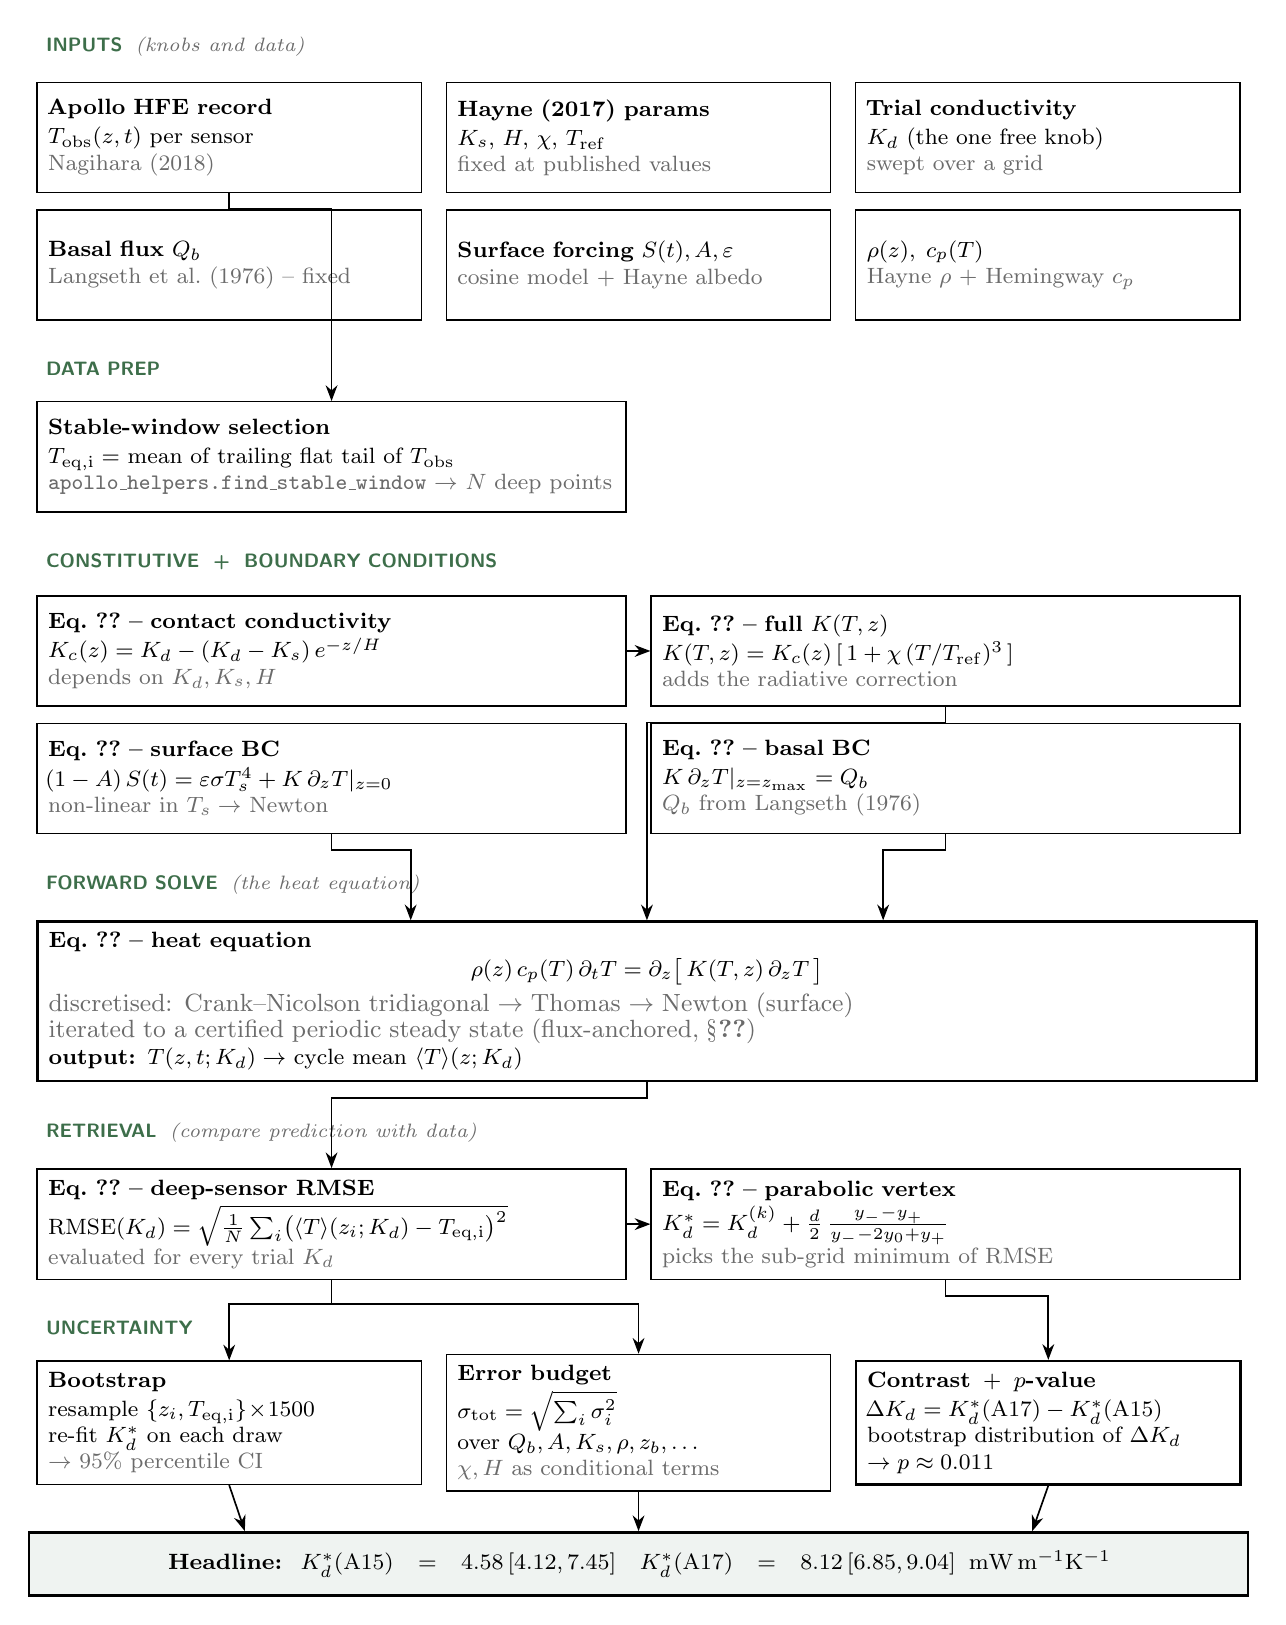
\begin{tikzpicture}[
  font=\footnotesize,
  every node/.style={align=left},
  box/.style={rectangle, draw=black, line width=0.5pt, inner sep=4pt,
              text width=46mm, minimum height=14mm, fill=white},
  wide/.style={text width=152mm},
  half/.style={text width=72mm},
  bandlabel/.style={font=\sffamily\bfseries\scriptsize\color{forest},
                    anchor=west},
  arr/.style={-{Stealth[length=2mm]}, line width=0.6pt}
]
% ---------- LEVEL 1: INPUTS ----------
\node[bandlabel] (L1) at (-78mm, 0) {INPUTS \;\textnormal{\color{dim}\itshape (knobs and data)}};
\node[box, below=2mm of L1.south west, anchor=north west] (in1)
  {\textbf{Apollo HFE record}\\[1pt]
   $T_{\rm obs}(z,t)$ per sensor\\
   {\color{dim}Nagihara (2018)}};
\node[box, right=3mm of in1] (in2)
  {\textbf{Hayne (2017) params}\\[1pt]
   $K_s,\,H,\,\chi,\,T_{\rm ref}$\\
   {\color{dim}fixed at published values}};
\node[box, right=3mm of in2] (in3)
  {\textbf{Trial conductivity}\\[1pt]
   $K_d$ (the one free knob)\\
   {\color{dim}swept over a grid}};
\node[box, below=2mm of in1] (in4)
  {\textbf{Basal flux $Q_b$}\\
   {\color{dim}Langseth et al.\ (1976) -- fixed}};
\node[box, below=2mm of in2] (in5)
  {\textbf{Surface forcing $S(t),A,\varepsilon$}\\
   {\color{dim}cosine model + Hayne albedo}};
\node[box, below=2mm of in3] (in6)
  {\textbf{$\rho(z),\;c_p(T)$}\\
   {\color{dim}Hayne $\rho$ + Hemingway $c_p$}};

% ---------- LEVEL 2: DATA PREP ----------
\node[bandlabel, below=4mm of in4.south west, anchor=north west] (L2)
  {DATA PREP};
\node[box, half, below=2mm of L2.south west, anchor=north west] (dp)
  {\textbf{Stable-window selection}\\[1pt]
   $T_{\rm eq,i}=$ mean of trailing flat tail of $T_{\rm obs}$\\
   {\color{dim}\texttt{apollo\_helpers.find\_stable\_window} $\to$ $N$ deep points}};
\draw[arr] (in1.south) -- ++(0,-2mm) -| (dp.north);

% ---------- LEVEL 3: CONSTITUTIVE + BC ----------
\node[bandlabel, below=4mm of dp.south west, anchor=north west] (L3)
  {CONSTITUTIVE\ \ +\ \ BOUNDARY CONDITIONS};
\node[box, half, below=2mm of L3.south west, anchor=north west] (eqKc)
  {\textbf{Eq.~\ref{eq:Kc} -- contact conductivity}\\[1pt]
   $K_c(z)=K_d-(K_d-K_s)\,e^{-z/H}$\\
   {\color{dim}depends on $K_d,K_s,H$}};
\node[box, half, right=3mm of eqKc] (eqK)
  {\textbf{Eq.~\ref{eq:Khayne} -- full $K(T,z)$}\\[1pt]
   $K(T,z)=K_c(z)\,[\,1+\chi\,(T/T_{\rm ref})^3\,]$\\
   {\color{dim}adds the radiative correction}};
\node[box, half, below=2mm of eqKc] (bcS)
  {\textbf{Eq.~\ref{eq:surfbc} -- surface BC}\\[1pt]
   $(1-A)\,S(t)=\varepsilon\sigma T_s^4+K\,\partial_z T|_{z=0}$\\
   {\color{dim}non-linear in $T_s\to$ Newton}};
\node[box, half, right=3mm of bcS] (bcB)
  {\textbf{Eq.~\ref{eq:bottombc} -- basal BC}\\[1pt]
   $K\,\partial_z T|_{z=z_{\max}}=Q_b$\\
   {\color{dim}$Q_b$ from Langseth (1976)}};
\draw[arr] (eqKc.east) -- (eqK.west);

% ---------- LEVEL 4: PDE ----------
\node[bandlabel, below=4mm of bcS.south west, anchor=north west] (L4)
  {FORWARD SOLVE \;\textnormal{\color{dim}\itshape (the heat equation)}};
\node[box, wide, below=2mm of L4.south west, anchor=north west,
      minimum height=20mm, line width=0.8pt] (pde) {%
  \textbf{Eq.~\ref{eq:heat} -- heat equation}\\[1pt]
  \hfill$\displaystyle \rho(z)\,c_p(T)\,\partial_t T=\partial_z\bigl[\,K(T,z)\,\partial_z T\,\bigr]$\hfill\null\\[2pt]
  {\color{dim}\small discretised: Crank--Nicolson tridiagonal $\to$ Thomas $\to$ Newton (surface)}\\
  {\color{dim}\small iterated to a certified periodic steady state (flux-anchored, \S\ref{sec:cert})}\\
  \textbf{output:} $T(z,t;K_d)\to$ cycle mean $\langle T\rangle(z;K_d)$};
\draw[arr] (eqK.south) -- ++(0,-2mm) -| (pde.north);
\draw[arr] (bcS.south) -- ++(0,-2mm) -| ($(pde.north)+(-30mm,0)$);
\draw[arr] (bcB.south) -- ++(0,-2mm) -| ($(pde.north)+(30mm,0)$);

% ---------- LEVEL 5: RETRIEVAL ----------
\node[bandlabel, below=4mm of pde.south west, anchor=north west] (L5)
  {RETRIEVAL \;\textnormal{\color{dim}\itshape (compare prediction with data)}};
\node[box, half, below=2mm of L5.south west, anchor=north west] (rmse)
  {\textbf{Eq.~\ref{eq:rmse} -- deep-sensor RMSE}\\[1pt]
   $\mathrm{RMSE}(K_d)=\sqrt{\tfrac{1}{N}\sum_i\bigl(\langle T\rangle(z_i;K_d)-T_{\rm eq,i}\bigr)^2}$\\
   {\color{dim}evaluated for every trial $K_d$}};
\node[box, half, right=3mm of rmse] (vertex)
  {\textbf{Eq.~\ref{eq:vertex} -- parabolic vertex}\\[1pt]
   $K_d^{*}=K_d^{(k)}+\tfrac{d}{2}\,\tfrac{y_--y_+}{y_--2y_0+y_+}$\\
   {\color{dim}picks the sub-grid minimum of RMSE}};
\draw[arr] (pde.south) -- ++(0,-2mm) -| (rmse.north);
\draw[arr] (rmse.east) -- (vertex.west);

% ---------- LEVEL 6: UNCERTAINTY ----------
\node[bandlabel, below=4mm of rmse.south west, anchor=north west] (L6)
  {UNCERTAINTY};
\node[box, below=2mm of L6.south west, anchor=north west] (boot)
  {\textbf{Bootstrap}\\[1pt]
   resample $\{z_i,T_{\rm eq,i}\}\!\times\!1500$\\
   re-fit $K_d^{*}$ on each draw\\
   {\color{dim}$\to$ 95\% percentile CI}};
\node[box, right=3mm of boot] (budg)
  {\textbf{Error budget}\\[1pt]
   $\sigma_{\rm tot}=\sqrt{\sum_i\sigma_i^2}$\\
   over $Q_b,A,K_s,\rho,z_b,\ldots$\\
   {\color{dim}$\chi,H$ as conditional terms}};
\node[box, right=3mm of budg, line width=0.8pt] (contr)
  {\textbf{Contrast \,$+$\, $p$-value}\\[1pt]
   $\Delta K_d=K_d^{*}({\rm A17})-K_d^{*}({\rm A15})$\\
   bootstrap distribution of $\Delta K_d$\\
   $\to p\approx 0.011$};
\draw[arr] (vertex.south) -- ++(0,-2mm) -| (contr.north);
\draw[arr] (rmse.south) -- ++(0,-3mm) -| (boot.north);
\draw[arr] (rmse.south) -- ++(0,-3mm) -| (budg.north);

% ---------- RESULT STRIP ----------
\node[draw=black, line width=1pt, fill=forest!8,
      text width=152mm, minimum height=8mm,
      below=5mm of budg.south, anchor=north,
      align=center, inner sep=4pt] (out)
  {\textbf{Headline:}\;
   $K_d^{*}({\rm A15})=4.58\,[4.12,7.45]$\quad
   $K_d^{*}({\rm A17})=8.12\,[6.85,9.04]$\;\;mW\,m$^{-1}$K$^{-1}$};
\draw[arr] (boot.south)  -- ($(out.north)+(-50mm,0)$);
\draw[arr] (budg.south)  -- (out.north);
\draw[arr] (contr.south) -- ($(out.north)+(50mm,0)$);
\end{tikzpicture}

\caption{Equation flow from inputs to $K_d^{*}$. Six raw inputs feed the
conductivity formulas (Eqs.~\ref{eq:Kc}--\ref{eq:Khayne}), which with the
boundary conditions define the heat equation (Eq.~\ref{eq:heat}). The forward
solve produces $\Tm(z;K_d)$, compared to the Apollo data through the deep-sensor
RMSE (Eq.~\ref{eq:rmse}); the parabolic vertex (Eq.~\ref{eq:vertex}) picks the
sub-grid minimum $K_d^{*}$. Uncertainty propagates downward: bootstrap CI,
quadrature budget, and the inter-site contrast with its $p$-value.}
\label{fig:eqnflow}
\end{figure}

\paragraph{\textbf{Step 1 --- read the Apollo HFE record.}}
On 31 July 1971 the Apollo~15 crew drilled two $\sim$2.4-m holes at Hadley Rille
and emplaced the Heat Flow Experiment (HFE): thin probes carrying
platinum-resistance temperature bridges at several depths. Apollo~17 carried a
similar, deeper pair. The probes recorded subsurface temperatures from 1971 to
1977. For $\sim$40 years the data sat on magnetic tape; in 2018 Nagihara et al.\
recovered and re-digitised the full record (with $\pm2.5$\,cm per-sensor depth
uncertainty). That restored record, read by \code{src/lunar/apollo\_helpers.py},
is our raw input.

\paragraph{\textbf{Step 2 --- extract $T_{\rm eq}$ from the stable window.}}
The instant the probes were emplaced they read $\sim$330\,K: the drill had heated
the borehole wall. For the next $\sim$2.7 years each sensor decayed exponentially
toward the undisturbed regolith temperature and then flattened. We do not trust
the early record. The code scans the trailing 55--85\% of each sensor's series
and picks the earliest window whose linear trend is flatter than
$0.08$\,K\,yr$^{-1}$; the mean of that quiet tail is the sensor's equilibrium
temperature $T_{\rm eq}$, and its scatter sets the noise. Only sensors below
80\,cm --- below the daily skin --- are kept: 7 at Apollo~15, 16 at Apollo~17.
These deep $(z,T_{\rm eq})$ dots are what the model must hit
(Fig.~\ref{fig:timeline}).

\begin{figure}[p]\centering

\includegraphics[width=\linewidth]{figures/fig_apollo_timeline.pdf}
\caption{Per-probe stability-window timeline for all four Apollo HFE probes.
\emph{Top of each block}: raw HFE traces; coral bands mark documented
data-quality events. Coloured rectangles are the accepted stability windows ---
the trailing flat tail with slope below $0.08$~K\,yr$^{-1}$. \emph{Below}: a
depth-ordered strip; each row's $T_{\rm eq}$ on the right is the mean over the
kept intervals. Grey rows are shallow sensors, excluded. Together these are the
23 deep $(z, T_{\rm eq})$ points the model must reproduce.}
\label{fig:timeline}
\end{figure}

\paragraph{\textbf{Step 3 --- choose a trial $K_d$.}}
$K_d$ is the one well-constrained unknown. Picture the column from the bottom up:
a small steady geothermal flux $Q_b\!\sim\!21$\,mW\,m$^{-2}$ (measured separately
by Langseth, held fixed) passes up through every layer. Where the regolith
conducts well the temperature changes little per metre; where it conducts poorly
the gradient steepens. So the deep gradient is just $Q_b/K_d$ --- and that is
exactly what the deep sensors see. $K_d$ is a property of the material, like
density, not a fudge factor. We will try many values and keep the one that fits.

\paragraph{\textbf{Step 4 --- build $K(T,z)$ and the density profile (Hayne).}}
Fixing the trial $K_d$ determines the whole conductivity surface, via
Hayne~(2017). Heat passes grain-to-grain through tiny contact patches; near the
surface grains are loosely packed (small $K_s$), deeper they compact, so the
contact part rises exponentially toward the deep asymptote $K_d$:
\begin{equation}
K_c(z) \;=\; K_d - (K_d - K_s)\,e^{-z/H},\qquad K_s = 0.74\!\times\!10^{-3},\quad H = 0.06\;\text{m}.
\label{eq:Kc}
\end{equation}
At daytime temperatures photons also hop across the empty pore spaces, a
radiative term rising as $T^3$:
\begin{equation}
K(T,z) \;=\; K_c(z)\,\bigl[\,1 + \chi\,(T/T_{\rm ref})^3\,\bigr],
\qquad \chi = 2.7,\quad T_{\rm ref}=350\;\text{K}.
\label{eq:Khayne}
\end{equation}
The same paper supplies $\rho(z)$ ($1100\!\to\!1800$\,kg\,m$^{-3}$); Hemingway
(1973) supplies $c_p(T)$; both conductivity terms are derived from their physics
in App.~\ref{app:hayne}. Fix the five Hayne constants and the density profile,
and the only free number left is $K_d$ (Fig.~\ref{fig:kTz}). That is what makes
this a one-parameter retrieval.

\begin{figure}[htbp]\centering
\includegraphics[width=0.82\linewidth]{figures/fig_book_kTz.pdf}
\caption{The Hayne conductivity $K(T,z)$. It rises with depth (compaction, via
$K_c$) and with temperature (radiation, via the $T^3$ bracket). Fixing every
constant except $K_d$ leaves a one-parameter family of surfaces; the retrieval
picks the member that fits the deep sensors.}
\label{fig:kTz}
\end{figure}

\paragraph{\textbf{Step 5 --- solve the heat equation forward.}}
With $K(T,z)$ chosen, we solve the heat equation in the column (derived in
App.~\ref{app:heateq}),
\begin{equation}
\rho\,c_p\,\frac{\partial T}{\partial t}
=\frac{\partial}{\partial z}\!\left(K\,\frac{\partial T}{\partial z}\right),
\label{eq:heat}
\end{equation}
closed by a radiative balance at the top --- sunlight absorbed equals infrared
radiated plus heat conducted downward,
\begin{equation}
(1-A)\,S(t) \;=\; \varepsilon\sigma T_s^4 \;+\; K_{\rm surf}\,\frac{T_s-T_{\rm sub}}{\Delta z_{\rm surf}/2},
\label{eq:surfbc}
\end{equation}
and by the fixed geothermal flux at the bottom (Langseth 1976),
\begin{equation}
K\,\frac{\partial T}{\partial z}\bigg|_{z_{\max}} \;=\; Q_b.
\label{eq:bottombc}
\end{equation}
Both boundary conditions are derived in App.~\ref{app:bc}. No closed-form
solution exists when $K$ depends on both $T$ and $z$, so we discretise: a
\emph{geometric} depth grid ($\Delta z_0=2$\,mm at the surface, each cell 8\%
thicker, 69 cells to $z_{\max}=5$\,m) and hourly time steps ($\Delta t=3600$\,s,
$\sim$709 per lunation). The grid follows one rule of thumb --- fine cells where
the temperature changes fast (millimetres at the surface, which sees a
$\sim$280\,K swing each lunation), coarse cells where it does not (tens of
centimetres by $1$\,m); App.~\ref{app:grid} gives the finite-volume cells and the
harmonic-mean face conductivities. The dimensionless cell-to-cell coupling per step,
$\alpha=\Delta t\,K/(\rho c_p\,\Delta z^2)$, stays small ($\sim10^{-3}$), so
neighbouring cells nudge each other only gently each hour. Three pieces of
machinery advance one hour, and they are all you need to understand the solver
(Fig.~\ref{fig:cnstencil}):

\begin{itemize}[leftmargin=1.4em,itemsep=3pt]
\item \textbf{Crank--Nicolson} sets the update rule. An \emph{explicit} scheme
  (use the old temperatures) is simple but unstable unless $\Delta t$ is
  absurdly small; an \emph{implicit} scheme (use the new temperatures) is stable
  but only first-order accurate. Crank--Nicolson averages the two: it is
  unconditionally stable \emph{and} second-order accurate. The picture is
  estimating a slope between two points by averaging the slopes at both
  endpoints, not just one. This couples all the new temperatures into one linear
  system $\mathbf{A}\,\mathbf{T}^{n+1}=\mathbf{d}$, and because each cell only
  talks to its immediate neighbours, $\mathbf{A}$ is \emph{tridiagonal} (nonzero
  only on three diagonals). Derived, with the truncation-error and stability
  arguments, in App.~\ref{app:cn}; the matrix assembly and boundary rows in
  App.~\ref{app:assembly}.
\item \textbf{The Thomas algorithm} solves that tridiagonal system in $O(N)$
  --- two sweeps (a forward elimination, a backward substitution) instead of the
  $\sim N^3/3$ of general Gaussian elimination. For 69 cells it is
  sub-microsecond (App.~\ref{app:thomas}).
\item \textbf{Newton's method} handles the surface. The top balance
  $(1-A)S(t)=\varepsilon\sigma T_s^4 + \text{(conduction down)}$ is non-linear in
  $T_s$ because of the $T_s^4$ infrared term. Newton slides along the tangent to
  the residual until it hits zero --- 2--3 iterations per hour. It runs
  \emph{every time step} (the insolation $S(t)$ changes hourly), and feeds its
  $T_s^{n+1}$ into the matrix as the top boundary value before Thomas solves
  (App.~\ref{app:newton}).
\end{itemize}

\begin{figure}[htbp]\centering
% Crank-Nicolson stencil: one cell at t^n and t^{n+1} with neighbours.
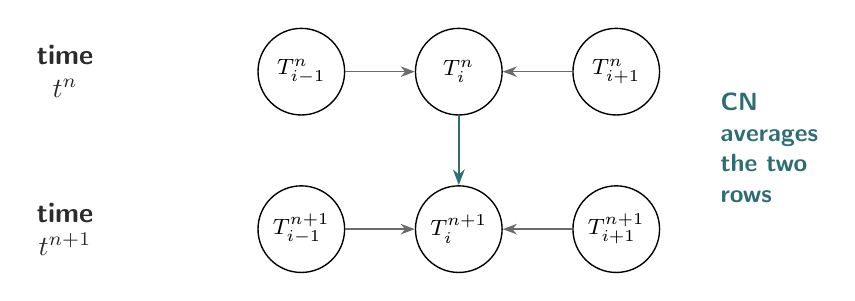
\begin{tikzpicture}[
  font=\footnotesize,
  node distance=18mm,
  T/.style={circle, draw=black, line width=0.5pt, fill=white,
            minimum size=11mm, inner sep=0pt,
            font=\footnotesize},
  arr/.style={-{Stealth[length=1.8mm]}, line width=0.5pt, color=dim},
  arrCN/.style={-{Stealth[length=2mm]}, line width=0.8pt, color=teal},
  every node/.style={align=center}
]
% Time axis label
\node[font=\sffamily\bfseries, color=char] at (-30mm, 0)
  {time\\$t^n$};
\node[font=\sffamily\bfseries, color=char] at (-30mm, -20mm)
  {time\\$t^{n+1}$};
% t^n row
\node[T] (Tnm1) at (0,0) {$T_{i-1}^{n}$};
\node[T] (Tni)  at (20mm,0) {$T_{i}^{n}$};
\node[T] (Tnp1) at (40mm,0) {$T_{i+1}^{n}$};
% t^{n+1} row
\node[T] (Tnp1m1) at (0,-20mm)  {$T_{i-1}^{n+1}$};
\node[T] (Tnp1i)  at (20mm,-20mm) {$T_{i}^{n+1}$};
\node[T] (Tnp1p1) at (40mm,-20mm) {$T_{i+1}^{n+1}$};
% Coupling arrows (lateral, t^n)
\draw[arr] (Tnm1.east) -- (Tni.west);
\draw[arr] (Tnp1.west) -- (Tni.east);
% Coupling arrows (lateral, t^{n+1})
\draw[arr] (Tnp1m1.east) -- (Tnp1i.west);
\draw[arr] (Tnp1p1.west) -- (Tnp1i.east);
% Vertical CN time-coupling
\draw[arrCN] (Tni.south) -- (Tnp1i.north);
% Annotation: half + half on the right
\node[anchor=west, color=teal, font=\sffamily\small\bfseries]
  at (52mm, -10mm)
  {\begin{tabular}{@{}l@{}}CN \\ averages\\ the two\\ rows\end{tabular}};
\end{tikzpicture}

\caption{The Crank--Nicolson stencil. Each new temperature $T_i^{n+1}$ is coupled
to its two neighbours at \emph{both} the old time level $t^n$ and the new level
$t^{n+1}$; CN averages the two rows. That symmetry is what buys unconditional
stability and second-order accuracy at once.}
\label{fig:cnstencil}
\end{figure}

\noindent Repeat the hour $\sim$709 times for one lunation and the \emph{thermal
skin wave} appears: the surface swings between $\sim$390\,K (noon) and
$\sim$100\,K (night), and that swing damps exponentially with depth, halving
every $\sim$6\,cm. By 80\,cm the daily wave is gone and only the slow geothermal
signal remains. (The detailed 5-cell worked example for all three pieces ---
matrix, sweeps, Newton step --- is in the extended edition; here we only need to
know what they do.)

\paragraph{\textbf{Step 6 --- run the flux-anchored loop to steady state.}}
One lunation is not enough. $K_d$ is a \emph{steady-state} property: only once
the deep column has stopped drifting does its gradient equal $Q_b/K_d$. Reaching
that state by brute time-stepping would take $\sim$1000 lunations (the diffusive
timescale of a 5\,m column) --- months of compute across the sweep and bootstrap.
Instead the solver alternates a short forward solve (settle the fast skin) with a
direct integration of the steady-state equation below an anchor depth (build the
slow deep column without waiting for diffusion). This is the methodological
centrepiece, and Ch.~\ref{ch:slope} is devoted to it. For the pipeline, the one
thing to hold onto: Step~6 turns a trial $K_d$ into a \emph{certified}
cycle-mean profile $\Tm(z;K_d)$ in $\sim$9\,s.

\paragraph{\textbf{Step 7 --- score the trial with RMSE.}}
The certified profile gives a model temperature at every depth. Interpolate it to
the real sensor depths, compare to the measured $T_{\rm eq}$, and collapse the
residuals into one number:
\begin{equation}
\mathrm{RMSE}(K_d)=\sqrt{\frac{1}{N}\sum_{i=1}^{N}\bigl[\Tm(z_i;K_d)-T^{\rm obs}_i\bigr]^2}.
\label{eq:rmse}
\end{equation}
One number that says how badly this trial fits the data.

\paragraph{\textbf{Step 8 --- sweep $K_d$ to a minimum.}}
Repeat Steps 4--7 across a grid of trial $K_d$ (28 values over $1$--$15$ at A15,
30 over $3$--$25$ at A17). Plotting RMSE versus $K_d$ gives a smooth bowl --- the
solver is deterministic and the steady state is unique for each $K_d$, so the
curve is clean (Fig.~\ref{fig:sweep}). The minimum is the best fit. We do not
want to round to the grid, so we fit a parabola through the three lowest points
and read its vertex:
\begin{equation}
K_d^{*}=K_d^{(k)}+\frac{\Delta}{2}\,\frac{y_--y_+}{y_--2y_0+y_+},
\label{eq:vertex}
\end{equation}
giving sub-grid precision with no extra (9-second) solves (App.~\ref{app:vertex}).
For Apollo~15 the
vertex sits at $K_d^{*}=4.58$\,mW\,m$^{-1}$K$^{-1}$ with RMSE $\approx0.95$\,K.

\begin{figure}[htbp]\centering

\includegraphics[width=0.82\linewidth]{figures/fig_kd_sweep.pdf}
\caption{Deep-sensor RMSE vs.\ trial $K_d$. Each site shows a clean single
minimum; Apollo~17's sits at a clearly higher conductivity than Apollo~15's. The
vertex of a parabola through the three lowest points is $K_d^{*}$.}
\label{fig:sweep}
\end{figure}

\paragraph{\textbf{Step 9 --- bootstrap for a confidence interval.}}
Seven dots, one number --- how confident are we? We cannot re-fly the mission, so
the bootstrap pretends we can (the plug-in principle behind this is justified in
App.~\ref{app:stats}). Treat the seven sensors as the population, draw
seven \emph{with replacement} (some appear twice, some not at all), jitter each
depth by $\mathcal{N}(0,2.5\,\mathrm{cm})$ to fold in Nagihara's positional
uncertainty, and re-fit $K_d^{*}$. Repeat 1500 times. The 2.5th and 97.5th
percentiles of the 1500 re-fits are the 95\% confidence interval:
$K_d^{*}(\mathrm{A15})\in[4.12,\,7.45]$. Crucially the 28 forward profiles are
computed once and cached --- each resample only re-selects which residuals enter
the RMSE, so the whole bootstrap costs seconds, not $1500\times$ the sweep.

\paragraph{\textbf{Step 10 --- the headline.}}
Run the same ten steps at Apollo~17 ($Q_b=15$, 16 sensors) and you get
$K_d^{*}(\mathrm{A17})=8.12\,[6.85,\,9.04]$. Subtract the two on each joint
bootstrap draw and the median contrast is $\Delta K_d=3.31$
($\sim$$1.8\times$), with tail probability $p\approx0.011$ under the null of
equal $K_d$. That is the headline of Ch.~\ref{ch:study}. The rest of this guide
explains the one step that made it possible (Ch.~\ref{ch:slope}), why it beats
the old way (Ch.~\ref{ch:bruteforce}), and what the number means
(Ch.~\ref{ch:result}).

% =====================================================================
\chapter{The slope method: deep regolith temperature without waiting for diffusion}\label{ch:slope}
% =====================================================================

This is the chapter to read slowly. Everything in the pipeline hangs on Step~6 ---
turning a trial $K_d$ into a \emph{certified} steady state --- and that step is
the contribution of this work. The name we use for it is the \textbf{slope
method}, because instead of waiting for heat to diffuse it computes the deep
temperature \emph{slope} directly and walks the profile down. We build it from
the ground up: why the old way is slow, why its convergence test lied, the one
insight that fixes it, the equation it integrates, and then the machinery, with
real numbers.

\section{Why brute force is slow}\label{sec:slow}

The Apollo deep sensors report temperatures that have stopped changing year to
year --- the column is in \emph{periodic steady state}, repeating identically
each lunation. $K_d$ is only readable there, because only in steady state does
the same conductive flux pass through every slab, making the deep gradient
exactly $Q_b/K_d$. Anything earlier still remembers the arbitrary starting guess.

How long must we time-step to forget that guess? The relevant time is the
\emph{diffusive timescale} for the column depth:
\begin{equation}
\tau \;\sim\; \frac{z_{\max}^2}{\kappa}
\;\sim\; \frac{(5\,\text{m})^2}{10^{-8}\,\text{m}^2/\text{s}}
\;\sim\; 2.5\!\times\!10^{9}\,\text{s}
\;\sim\; 80\ \text{years}
\;\sim\; 1000\ \text{lunations}.
\label{eq:tau}
\end{equation}
\emph{Where this comes from.} Balance the heat equation by dimensions: the
storage term $\partial_t T\sim T/\tau$ against $\kappa\,\partial_z^2 T\sim\kappa
T/L^2$, so the time to diffuse across a length $L$ is $\tau\sim L^2/\kappa$. The
quadratic in $L$ is the whole story, and it splits the column cleanly in two: a
thin skin of thickness $\ell\sim20$\,cm settles in
$\tau_{\rm skin}\sim\ell^2/\kappa\sim$ a few lunations, while the full $5$\,m
column takes $(5/0.2)^2\approx600$ times longer --- of order $10^3$ lunations.
That factor of $\sim$600 between the fast skin and the slow column is exactly the
trap the next section springs.

Picture the approach as a damped exponential: the deep column halves its
remaining error every $\sim$10 lunations. Starting $\sim$25\,K from the truth, reaching $0.05$\,K takes about
nine halvings --- $\sim$90 lunations just to \emph{almost} converge, and far more
to nail it. At 9~s per lunation, that is hours per trial $K_d$; across 28 trials,
2 sites, and 1500 bootstraps, brute force runs to months. It does not scale.

\section{The F1 bug: convergence that wasn't}\label{sec:f1}

The literature spin-up sidestepped this by running a fixed 30 lunations and
checking ``has the cycle-to-cycle change dropped below $0.01$\,K?''. By 30
lunations that test always passed --- but only because the thin \emph{skin} had
equilibrated (it settles in $\sim$10 lunations, since
$\tau_{\rm skin}\sim\ell^2/\kappa$ with $\ell\!\sim\!20$\,cm). The deep column
was still 10--40\,K from its true value, drifting so slowly
($\sim$$10^{-3}$\,K/lunation) that the cycle-to-cycle change was already under
threshold. The test measured whether progress had \emph{slowed}, not whether the
profile had \emph{arrived}. We call this flag F1.

\begin{plain}
Picture a puddle next to a lake. The puddle settles in seconds; the lake takes
hours. If you only watch the puddle, you declare ``calm'' as soon as the ripples
stop --- while the lake is still draining. The 30-lunation test watched the
puddle (the skin) when the lake (the deep column) was the part that mattered.
\end{plain}

\noindent The consequence is fatal for the retrieval: the deep sensors at
0.8--2.4\,m sit exactly in the unsettled zone, so their modelled temperatures
depend partly on $K_d$ and partly on the starting guess. Initialise at 240\,K and
you get one $K_d$; at 260\,K, another. The starting guess had become a hidden
free parameter (Fig.~\ref{fig:f1bug}).

\begin{figure}[htbp]\centering
\includegraphics[width=\linewidth]{figures/fig_book_f1_bug.pdf}
\caption{Why flag F1 fooled the old solver.}
\label{fig:f1bug}
\end{figure}
\begin{figdesc}
\textbf{(a)} The cycle-to-cycle change (teal) drops below the old $0.01$\,K
tolerance long before the true deep-profile error (coral) does; by 30 lunations
the test passes but the deep column is still tens of kelvin off. \textbf{(b)} At
the sensor depths (shaded band), a fixed 30-lunation spin-up depends on the
starting guess --- two guesses (240\,K, 260\,K) land on visibly different
profiles. The flux-anchored fix lands on the true profile (dashed) from either
start.
\end{figdesc}

\section{The key insight}\label{sec:insight}

The fix observes that the slow part --- the deep column's drift --- does not
actually require time integration at all. In steady state the deep temperature
obeys a simple first-order ODE in depth (derived in App.~\ref{app:closure}):
\begin{equation}
\frac{d\Tm}{dz} \;=\; \frac{Q_b - u_{\rm rect}(z)}{K(\Tm,\,z)}.
\label{eq:closure}
\end{equation}
At any depth, the slope is the flux ($Q_b$, known, plus a small correction
$u_{\rm rect}$) divided by the conductivity at that depth (computable once we
know the temperature there). So if we know the temperature at \emph{one} depth
below the skin, we can compute the next depth down, and the next --- building the
entire deep profile by walking down the slope, never simulating the slow
diffusion. The one temperature we need is the \textbf{anchor}: the cycle-mean
temperature at a depth $z_0$ just below the daily skin, where the skin has
already settled (the skin-depth scale $\delta$ is derived in App.~\ref{app:skin}).
The whole method is two operations, alternated
(Fig.~\ref{fig:fluxanchored}):

\begin{itemize}[leftmargin=1.4em,itemsep=3pt]
\item \textbf{Step A --- forward solve.} From the current guess of the cycle-mean
  profile, run a few lunations of hour-by-hour Crank--Nicolson+Newton+Thomas.
  The fast skin settles into its true oscillation. Read off the anchor
  temperature $\Tm(z_0)$ and the rectified flux $u_{\rm rect}(z)$.
\item \textbf{Step B --- closure reconstruction.} From the anchor, integrate
  Eq.~\eqref{eq:closure} downward (RK2). This rebuilds the deep profile in
  microseconds.
\end{itemize}
\noindent Set the guess to the reconstruction and repeat. When the anchor
temperature stops moving by more than $0.005$\,K, declare convergence --- 6--10
cycles, $\sim$9\,s per trial $K_d$.

\begin{figure}[htbp]\centering
% Flux-anchored equilibrium loop: Step A -> Step B -> closure.
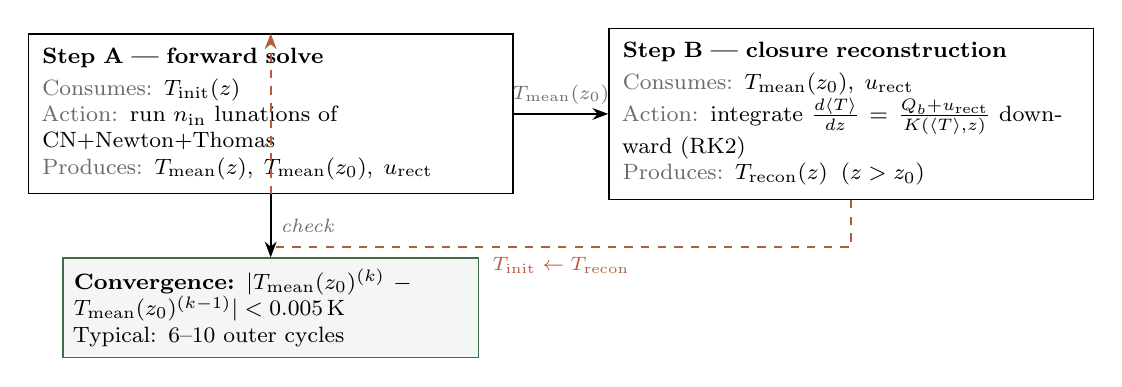
\begin{tikzpicture}[
  font=\footnotesize,
  every node/.style={align=left},
  bx/.style={rectangle, draw=black, line width=0.6pt, fill=white,
             inner sep=5pt, text width=58mm, minimum height=20mm,
             anchor=north west},
  result/.style={rectangle, draw=forest, line width=0.6pt, fill=forest!6,
                 inner sep=4pt, text width=50mm, minimum height=10mm,
                 anchor=north west},
  arr/.style={-{Stealth[length=2mm]}, line width=0.6pt},
  loop/.style={-{Stealth[length=2mm]}, line width=0.7pt, color=coral, dashed}
]
\node[bx] (A) at (0,0)
  {\textbf{Step A --- forward solve}\\[2pt]
   {\color{dim}Consumes:} $T_{\rm init}(z)$\\
   {\color{dim}Action:} run $n_{\rm in}$ lunations of CN+Newton+Thomas\\
   {\color{dim}Produces:} $T_{\rm mean}(z),\;T_{\rm mean}(z_0),\;u_{\rm rect}$};
\node[bx, right=12mm of A] (B)
  {\textbf{Step B --- closure reconstruction}\\[2pt]
   {\color{dim}Consumes:} $T_{\rm mean}(z_0),\;u_{\rm rect}$\\
   {\color{dim}Action:} integrate
   $\frac{d\langle T\rangle}{dz}=\frac{Q_b+u_{\rm rect}}{K(\langle T\rangle,z)}$
   downward (RK2)\\
   {\color{dim}Produces:} $T_{\rm recon}(z)\;\;(z>z_0)$};
\node[result, below=8mm of A] (R)
  {\textbf{Convergence:} $|T_{\rm mean}(z_0)^{(k)} - T_{\rm mean}(z_0)^{(k-1)}| < 0.005$\,K\\
   Typical: $6$--$10$ outer cycles};
% A -> B arrow
\draw[arr] (A.east) -- (B.west)
  node[midway, above, font=\scriptsize\itshape, color=dim]
  {$T_{\rm mean}(z_0)$};
% B -> A loopback (dashed coral)
\draw[loop] (B.south) -- ++(0,-6mm) -| (A.north)
  node[pos=0.25, below, font=\scriptsize\itshape, color=coral]
  {$T_{\rm init}\leftarrow T_{\rm recon}$};
% A -> R (when converged)
\draw[arr] (A.south) -- (R.north)
  node[pos=0.5, right, font=\scriptsize\itshape, color=dim]
  {check};
\end{tikzpicture}

\caption{The flux-anchored equilibrium loop. Step~A consumes the current
cycle-mean guess and runs a short forward solve, returning the anchor
temperature and $u_{\rm rect}$. Step~B integrates the steady closure equation
downward from the anchor, returning the deep profile. The dashed arrow closes
the loop; convergence is reached when the anchor temperature stops moving by more
than $0.005$\,K (typically 6--10 cycles).}
\label{fig:fluxanchored}
\end{figure}

\section{Where the closure equation comes from}\label{sec:closure}

Equation~\eqref{eq:closure} is the heart of the method, so here is its
derivation. Picture a deep parcel of regolith over one full lunation: the
temperature oscillates but returns exactly to itself a lunation later (the
definition of periodic steady state). Time-average the heat equation
(Eq.~\eqref{eq:heat}) over that lunation:
\[
\Bigl\langle \rho c_p\,\partial_t T\Bigr\rangle
\;=\;
\Bigl\langle \partial_z\bigl(K\,\partial_z T\bigr)\Bigr\rangle.
\]
The left side averages to \emph{zero}: every bit of warming during the lunar day
is exactly cancelled by cooling during the night. The right side is a $z$-
derivative of a time average, so the average passes through: $\partial_z\langle
K\partial_z T\rangle=0$. Integrate once in $z$ and use the basal condition
$\langle K\partial_z T\rangle|_{z_{\max}}=Q_b$:
\begin{equation}
\bigl\langle K(T,z)\,\partial_z T\bigr\rangle \;=\; Q_b
\qquad\text{at every depth.}
\label{eq:fluxsame}
\end{equation}
In plain words: \emph{the cycle-mean conductive flux is the same at every depth
and equals the geothermal flux}. That is what ``the column carries $Q_b$ in
steady state'' means. To turn this into a slope we must peel apart the average ---
and because $K$ depends on $T$, and $T$ oscillates, $\langle K\partial_z
T\rangle \ne K(\Tm)\,\partial_z\Tm$ in general. Name the difference the
\textbf{rectified flux}:
\[
u_{\rm rect}(z) \;\equiv\;
\bigl\langle K(T,z)\,\partial_z T\bigr\rangle \;-\; K(\Tm,z)\,\partial_z\Tm.
\]
Substitute and rearrange, and Eq.~\eqref{eq:closure} drops out. The closure has
just two ingredients: the known $Q_b$ (a number from Langseth) and $u_{\rm rect}$
(computed once per outer cycle as a by-product of Step~A's cycle mean).

\section{Why $u_{\rm rect}$ exists, and why it is small}

The conductivity $K(T,z)$ depends on temperature, mostly through the radiative
$\chi(T/T_{\rm ref})^3$ term. When $T(t)$ swings by $\Delta T$ around its mean,
$K$ swings too, and the swing of $K$ correlates with the swing of the gradient
$\partial_z T$ in a way that does not average out --- that residual is
$u_{\rm rect}$. Quantitatively, expand $K$ about the mean: a swing $\Delta T$
produces $\Delta K\sim\tfrac12 K''(\Tm)\,\Delta T^2$ (the linear term averages
away; the curvature term does not), and multiplying that by the oscillating
gradient and time-averaging leaves a non-zero eddy flux. It is biggest where
$\Delta T$ is biggest: the top $\sim$30\,cm,
where it can reach $\sim$0.5\% of $Q_b$. Below the skin $\Delta T<1$\,K and
$u_{\rm rect}\to0$. That is precisely why the production anchor sits at
$z_0=0.55$\,m --- below the rectification zone, where the closure is simply
$d\Tm/dz=Q_b/K$.

\section{Step A, hour by hour}\label{sec:stepA}

Step~A is the forward solver of \S\,Step~5 run for $n_{\rm in}$ lunations. Think
of it as a state machine carrying just the temperature vector $T^n$ (69 numbers),
the surface temperature $T_s^n$, and the running sums needed for the cycle mean.
Each hour runs three sub-operations in order (\code{src/lunar/solver.py},
\code{\_step}):

\begin{enumerate}[leftmargin=1.4em,itemsep=3pt]
\item \textbf{Freeze material properties at $T^n$.} Evaluate $K,\rho,c_p$ at the
  old temperature. This linearisation costs nothing: with the coupling
  $\alpha\ll1$, $K$ changes by far less than a percent in one hour.
\item \textbf{Newton at the surface.} With $T_{\rm sub}=T_0^n$, solve
  $(1-A)S(t)-\varepsilon\sigma T_s^4 - K_{\rm surf}(T_s-T_{\rm sub})/(\Delta z_0/2)=0$
  to $10^{-4}$\,K --- 2--3 iterations.
\item \textbf{Assemble the tridiagonal system and run Thomas.} Build
  $a_i,b_i,c_i,d_i$ from $T^n$, modify row~0 (surface ghost from Newton's
  $T_s^{n+1}$) and row $n{-}1$ (basal ghost from $Q_b$), solve once for
  $T^{n+1}$.
\end{enumerate}

\noindent Nothing is carried between hours except the temperature state and the
running sums: the matrix is rebuilt each hour (because $K$ depends on the current
$T$), and Newton restarts each hour (because $S(t)$ has moved). After
$n_{\rm in}$ lunations Step~A returns three things for Step~B: the cycle mean
$\Tm(z)$, the anchor value $\Tm(z_0)$, and $u_{\rm rect}(z)$. Wall-clock cost:
$\sim$9\,s, JIT-compiled.

\section{One Crank--Nicolson hour, worked}\label{sec:cnhour}

The three sub-operations are abstract until you watch them move real numbers, so
do one hour by hand on the 5-cell toy of Fig.~\ref{fig:toy}: uniform
$\Delta z=0.10$\,m, $K=10$\,mW\,m$^{-1}$K$^{-1}$, volumetric heat capacity
$\rho c_p=9\!\times\!10^{5}$, so each cell's heat capacity per area is
$C=\rho c_p\,\Delta z=9\!\times\!10^{4}$ and the coupling is
\[
\alpha=\frac{\Delta t\,K}{\Delta z\,C}=\frac{3600\times0.010}{0.10\times9\!\times\!10^{4}}=4\!\times\!10^{-3}.
\]
Read $\alpha$ as ``how hard does a cell pull its neighbour in one hour?'' --- here,
very gently. Collecting every $T^{n+1}$ on the left, the CN update for an interior
cell is
\[
-\tfrac12\alpha\,T_{i-1}^{n+1}+(1+\alpha)\,T_i^{n+1}-\tfrac12\alpha\,T_{i+1}^{n+1}
=\tfrac12\alpha\,T_{i-1}^{n}+(1-\alpha)\,T_i^{n}+\tfrac12\alpha\,T_{i+1}^{n},
\]
so each row carries coefficients $(-0.002,\,1.004,\,-0.002)$ --- tridiagonal,
because a cell two rows away contributes nothing in one step.

\begin{figure}[htbp]\centering
% The 5-cell toy column used throughout §1.6 tutorial.
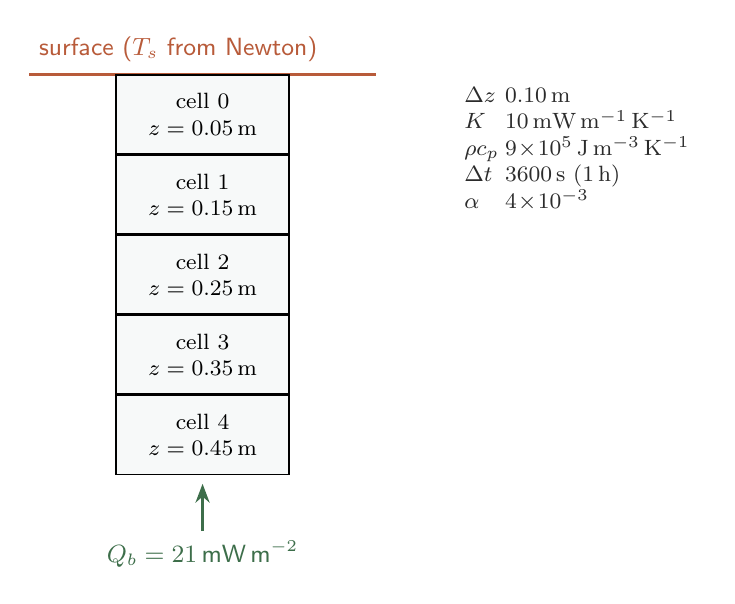
\begin{tikzpicture}[
  font=\footnotesize,
  cell/.style={rectangle, draw=black, line width=0.5pt,
               minimum width=22mm, minimum height=10mm, fill=teal!4,
               anchor=north},
  surfline/.style={line width=1.2pt, color=coral},
  basalarrow/.style={-{Stealth[length=2.4mm]}, line width=0.9pt, color=forest},
  every node/.style={align=center}
]
% Surface line above cell 0
\draw[surfline] (-22mm,0) -- (22mm,0);
\node[anchor=south west, color=coral, font=\sffamily\small]
  at (-22mm, 1pt) {surface  ($T_s$ from Newton)};
% The 5 cells
\node[cell] (c0) at (0,0)         {cell 0\\$z=0.05$\,m};
\node[cell, below=0mm of c0]  (c1)        {cell 1\\$z=0.15$\,m};
\node[cell, below=0mm of c1]  (c2)        {cell 2\\$z=0.25$\,m};
\node[cell, below=0mm of c2]  (c3)        {cell 3\\$z=0.35$\,m};
\node[cell, below=0mm of c3]  (c4)        {cell 4\\$z=0.45$\,m};
% Basal flux arrow rising from below
\draw[basalarrow] (0,-58mm) -- (0,-52mm);
\node[anchor=north, color=forest, font=\sffamily\small]
  at (0,-58mm) {$Q_b = 21$\,mW\,m$^{-2}$};
% Properties box on the right
\node[anchor=north west, font=\footnotesize, color=char]
  at (32mm, 0) {
    \begin{tabular}{@{}l@{\;}l@{}}
    $\Delta z$        & $0.10$\,m \\
    $K$               & $10$\,mW\,m$^{-1}$\,K$^{-1}$ \\
    $\rho c_p$        & $9\!\times\!10^{5}$\,J\,m$^{-3}$\,K$^{-1}$ \\
    $\Delta t$        & $3600$\,s ($1$\,h) \\
    $\alpha$          & $4\!\times\!10^{-3}$ \\
    \end{tabular}
  };
\end{tikzpicture}

\caption{The 5-cell toy column. The surface temperature comes from the Newton
solve; the basal flux $Q_b$ enters at the bottom. It is used twice: for one
worked Crank--Nicolson hour (this section) and for the Step~B downward walk
(\S\ref{sec:stepB}).}
\label{fig:toy}
\end{figure}

\noindent Start the toy uniform at $250$\,K. The boundary conditions are \textbf{four edits, nothing
more}: \emph{Newton at the surface} returns $T_s^{n+1}\approx372$\,K at midday
($S\approx1221$\,W\,m$^{-2}$) and enters row 0 only through its right-hand side,
$d_0\to d_0-\tfrac12\alpha T_0^n+\tfrac12\alpha(T_s^n+T_s^{n+1})\approx250.99$;
the \emph{basal ghost cell} carries $Q_b$ into row 4 by subtracting
$\tfrac12\alpha$ from the last diagonal ($b_4=1.004\to1.002$) and adding the flux
to the RHS ($d_4=250+\Delta t\,Q_b/C\approx250.00084$). The system is then
\[
\begin{bmatrix}
1.004 & -0.002 & & & \\
-0.002 & 1.004 & -0.002 & & \\
 & -0.002 & 1.004 & -0.002 & \\
 & & -0.002 & 1.004 & -0.002 \\
 & & & -0.002 & \mathbf{1.002}
\end{bmatrix}\mathbf{T}^{n+1}=
\begin{bmatrix}\mathbf{250.99}\\250\\250\\250\\\mathbf{250.00084}\end{bmatrix},
\]
the bold entries the only ones the boundaries touched. Now \textbf{Thomas}: the
forward sweep replaces each $(b_i,d_i)$ by modified $(c_i',d_i')$,
\begin{center}\small
\begin{tabular}{@{}cccc@{}}
\toprule
$i$ & $b_i-a_ic_{i-1}'$ & $c_i'$ & $d_i'$ \\
\midrule
0 & 1.004    & $-0.001992$ & 249.988 \\
1 & 1.003996 & $-0.001992$ & 249.503 \\
2 & 1.003996 & $-0.001992$ & 249.503 \\
3 & 1.003996 & $-0.001992$ & 249.503 \\
4 & 1.001996 & ---         & 249.999 \\
\bottomrule
\end{tabular}
\end{center}
and backward substitution from the bottom up gives
\[
\mathbf{T}^{n+1}=[\,250.486,\;250.001,\;250.001,\;250.001,\;249.999\,]\;\text{K}.
\]
The surface cell warmed $\sim$0.49\,K (it sits next to the 372\,K surface, and the
implicit half-step hands it about half the conductive pull); the middle cells
barely moved (one hour is far too short for heat to reach them); the deepest cell
gained $\sim$0.001\,K from the basal flux. That is one hour. Step~A is this hour
repeated $\sim$709 times per lunation for $\sim$12 lunations --- and \emph{that} is
the whole forward solve the slope method leans on.

\section{Step B as RK2 --- walking the deep profile down}\label{sec:stepB}

Step~B integrates the closure ODE from the anchor down to $z_{\max}$ by the
midpoint rule (Runge--Kutta order 2; its $O(\Delta z^3)$ local error is shown in
App.~\ref{app:rk2}), one cell at a time. To see it concretely,
walk the same toy column (Fig.~\ref{fig:toy}) with anchor at $z_0=0.05$\,m,
$K=10$\,mW\,m$^{-1}$K$^{-1}$ (taken constant for clarity),
$Q_b=21$\,mW\,m$^{-2}$, $u_{\rm rect}\approx0$ (we are below the skin), and
suppose Step~A returned $\Tm(z_0)=253.40$\,K. The step from cell $i$ to cell
$i{+}1$ is:

\begin{enumerate}[leftmargin=1.4em,itemsep=3pt]
\item \emph{Slope at the start of the cell:}
  $s_i = (Q_b-u_{{\rm rect},i})/K(\Tm_i,z_i)= 0.021/0.010 = 2.10$\,K\,m$^{-1}$.
\item \emph{Predict at the midpoint:}
  $\Tm_{i+1/2} = \Tm_i + (\Delta z/2)\,s_i = 253.40 + 0.05\times2.10 = 253.505$\,K.
\item \emph{Slope at the midpoint:}
  $s_{i+1/2} = (Q_b-u_{{\rm rect},i+1/2})/K(\Tm_{i+1/2},z_{i+1/2}) \approx 2.10$\,K\,m$^{-1}$.
\item \emph{Step using the midpoint slope:}
  $\Tm_{i+1} = \Tm_i + \Delta z\,s_{i+1/2} = 253.40 + 0.10\times2.10 = 253.61$\,K.
\end{enumerate}

\noindent Repeat cell by cell to the bottom. With $K$ taken constant here the
slope is $2.10$\,K\,m$^{-1}$ at every step (RK2 is then exact), so each $0.10$\,m
cell adds $0.21$\,K:

\begin{center}\small
\begin{tabular}{@{}cccccc@{}}
\toprule
$i$ & $z_i$ (m) & $\Tm_i$ (K) & slope $s_i$ (K\,m$^{-1}$) & $\Tm_{i+1/2}$ (K) & $\Tm_{i+1}$ (K) \\
\midrule
0 & 0.05 & 253.40 & 2.10 & 253.505 & 253.61 \\
1 & 0.15 & 253.61 & 2.10 & 253.715 & 253.82 \\
2 & 0.25 & 253.82 & 2.10 & 253.925 & 254.03 \\
3 & 0.35 & 254.03 & 2.10 & 254.135 & 254.24 \\
4 & 0.45 & 254.24 & --- & --- & --- \\
\bottomrule
\end{tabular}
\end{center}

\noindent The whole walk is five evaluations of $K$ and four cell-to-cell slopes
--- the deep column rebuilds itself in microseconds. In the real solver $K(\Tm,z)$
rises with depth, so the slope shrinks slightly cell to cell and the column curves
gently rather than running perfectly straight; the arithmetic is identical. The
real code (\code{\_reconstruct\_subskin},
\code{src/lunar/equilibrium.py:100}) is identical except it loops over $\sim$60
cells and uses the true depth- and temperature-dependent $K(\Tm,z)$ at each step:

\begin{lstlisting}[style=py]
T_new = T_mean.copy()                    # keep the skin as-is from Step A
for i in range(i0, N-1):                 # walk downward from the anchor
    dz = z[i+1] - z[i]
    q  = Q_b - u_rect[i]                 # flux minus the small eddy correction
    Ki = K(T_new[i], z[i])               # conductivity here
    T_half = T_new[i] + 0.5*q/Ki*dz      # RK2 midpoint
    K_half = K(T_half, 0.5*(z[i]+z[i+1]))
    T_new[i+1] = T_new[i] + q/K_half*dz  # THE STEP: T_next = T_here + slope*dz
\end{lstlisting}

\begin{plain}
The part people find hardest to believe is that we know the deep temperature
\emph{without simulating} it. In steady state, energy conservation fixes the
answer: the same $Q_b$ watts flow through every layer, and Fourier's law turns
that flux into a slope. So we walk downward adding ``slope $\times$ step.'' It is
exactly like finding elevation on a hill --- know one point and the slope
everywhere, and you can compute the height anywhere.
\end{plain}

\begin{figure}[htbp]\centering

\includegraphics[width=\linewidth]{figures/reconstruct_filmstrip.pdf}
\caption{Step~B as snapshots. From the anchor at 0.55\,m (the dot), the code
walks downward computing $d\Tm/dz=(Q_b-u_{\rm rect})/K$ at each depth. By the
fourth panel the entire deep profile is built, matching the true steady state
(dashed).}
\label{fig:reconstruct}
\end{figure}

\section{The outer loop as a fixed-point search}\label{sec:fixedpoint}

Steps A and B together define an operator on profiles:
\[
T_{\rm init}(z)\;\xrightarrow{\;\text{A}\;}\;\bigl(\Tm(z),\;u_{\rm rect}(z)\bigr)
\;\xrightarrow{\;\text{B}\;}\;T_{\rm recon}(z),
\]
and we set $T_{\rm init}\leftarrow T_{\rm recon}$ and repeat. Convergence is a
\emph{fixed point}: $T_{\rm init}=T_{\rm recon}$. Why does a unique one exist?
Two contracting properties:
\begin{itemize}[leftmargin=1.4em,itemsep=2pt]
\item \textbf{A is contractive on the skin.} Any starting profile, however wrong,
  relaxes toward the true skin solution within $\sim$3 lunations of Step~A,
  because the skin diffusive timescale is short.
\item \textbf{B is exact below the anchor.} The ODE Step~B integrates \emph{is}
  the steady-state equation, not an approximation. Given a correct anchor, B
  returns the true deep profile in one application.
\end{itemize}
Composed, $B\circ A$ pulls every starting profile toward the unique fixed point
where the skin matches the average of the forward solves \emph{and} the deep
column matches its own steady-state ODE. That fixed point \emph{is} the periodic
steady state. (Ch.~\ref{ch:bruteforce} confirms this empirically: it agrees with
a fully converged brute-force run to sub-millikelvin.)

\section{A full solve, cycle by cycle}\label{sec:fullsolve}

Putting Steps A and B together, here is what a complete Apollo~15 solve at
$K_d=4.58$ looks like from the outside. Start from a deliberately wrong flat
guess; each outer cycle settles the skin (A) and rebuilds the deep column (B),
and the anchor temperature --- the one number the loop watches --- contracts
toward its fixed value. The real trace --- read straight from the solver's
convergence history --- is (Fig.~\ref{fig:anchorconv}):

\begin{center}\small
\begin{tabular}{@{}clcc@{}}
\toprule
Stage & cycle & $\Tm(z_0)$ (K) & drift (K) \\
\midrule
1 ($z_0{=}0.25$\,m) & 1 & 250.99 & --- \\
                    & 2 & 250.93 & 0.063$^{\dagger}$ \\
\midrule
2 ($z_0{=}0.55$\,m) & 1 & 251.71 & --- \\
                    & 2 & 251.75 & 0.045 \\
                    & 3 & 251.78 & 0.028 \\
                    & 4 & 251.80 & 0.017 \\
                    & 5 & 251.81 & 0.010 \\
                    & 6 & 251.82 & 0.0062 \\
                    & 7 & 251.82 & 0.0038$^{\ddagger}$ \\
\bottomrule
\end{tabular}
\end{center}
\noindent{\footnotesize $^{\dagger}$ below the stage-1 tolerance ($0.10$\,K) ---
advance to the deeper anchor.\quad $^{\ddagger}$ below the stage-2 tolerance
($0.005$\,K) --- converged.}

\smallskip
\noindent In stage 2 the drift shrinks by about $40\%$ each cycle (geometric
ratio $\sim$0.6) --- the contraction the fixed-point argument guarantees. Nine
outer cycles, each a $\sim$9--12\,s Step~A plus a microsecond Step~B, take the
anchor to a $\sim$4\,mK drift, and the certified solve then passes all three
checks of \S\ref{sec:cert}. Run the \emph{same} loop from a 240\,K guess instead
of 260\,K and it lands within $0.038$\,K of this profile at every depth --- the
guess-independence number. Figure~\ref{fig:newfilm} shows the same solve as
snapshots: the skin settles, then Step~B snaps the deep column onto the steady
gradient.

\begin{figure}[htbp]\centering
\includegraphics[width=0.86\linewidth]{figures/fig_anchor_convergence.pdf}
\caption{What the anchor method actually does, one real Apollo~15 $K_d=4.58$
solve. \emph{Top:} the anchor temperature $\Tm(z_0)$ settling --- two cheap
shallow cycles ($z_0=0.25$\,m), then the deep stage ($z_0=0.55$\,m) refining to
$251.82$\,K. \emph{Bottom:} the inter-cycle drift contracting geometrically past
the stage-1 ($0.10$\,K) and stage-2 ($0.005$\,K) tolerances, reaching $3.8$\,mK
by the ninth cycle. This is the output the old fixed spin-up could never
certify.}
\label{fig:anchorconv}
\end{figure}

\begin{figure}[htbp]\centering

\includegraphics[width=\linewidth]{figures/newmethod_filmstrip.pdf}
\caption{The slope method as snapshots. Start from a deliberately wrong flat
guess (240\,K). Step~A settles the skin; Step~B's reconstruction snaps the deep
profile onto the steady gradient. After a few outer cycles the profile matches
the true steady state (dashed). Total cost: $\sim$150 lunations of stepping
($\sim$9\,s), versus $\sim$1000$+$ lunations for brute force.}
\label{fig:newfilm}
\end{figure}

\section{Why two anchor stages, not one}\label{sec:twostage}

The code runs the loop in two stages with different anchor depths
(\code{src/lunar/equilibrium.py:198}):
\begin{center}\small
\begin{tabular}{@{}lcccc@{}}
\toprule
Stage & anchor $z_0$ & $n_{\rm in}$ & max outer & tolerance \\
\midrule
1 (shallow) & $0.25$ m & 4 lunations  & 4 iterations  & $0.10$ K \\
2 (deep)    & $0.55$ m & 12 lunations & 20 iterations & $0.005$ K \\
\bottomrule
\end{tabular}
\end{center}

\noindent The rectified flux $u_{\rm rect}$ is concentrated in the top
$\sim$30\,cm. Anchor inside that zone and you integrate through a layer where
$u_{\rm rect}$ is large and carries the bias of a not-yet-converged Step~A ---
fast but slightly biased. So stage~1 \emph{uses} that on purpose: a shallow
anchor at 0.25\,m with short 4-lunation runs drags the bulk of the deep column
into the right ballpark cheaply (loose 0.10\,K tolerance, because stage~2 will
tighten it). Stage~2 then drops the anchor to 0.55\,m, comfortably below the
daily wave where $u_{\rm rect}\approx0$, and runs 12-lunation inner solves long
enough for the skin to fully equilibrate, closing the residual at a ten-times
tighter $0.005$\,K. In plain words: stage~1 gets you to the right neighbourhood
cheaply; stage~2 polishes you to the final number.

\section{Certification --- three checks, with real numbers}\label{sec:cert}

When the loop thinks it has converged, the solver runs three diagnostics
(\code{\_mean\_flux\_closure}, \code{src/lunar/equilibrium.py:139}). None of them
is the F1 trap (cycle-to-cycle change), and none can be passed by accident. For
the certified $K_d=4.58$ solve at Apollo~15:

\begin{center}\small
\begin{tabular}{@{}lccc@{}}
\toprule
Check & Quantity measured & Threshold & Observed \\
\midrule
Guess-independence & $\max_z|T_{(240)}(z)-T_{(260)}(z)|$  & $\le 0.05$ K   & $0.038$ K \\
Flux closure       & $|K\,d\Tm/dz - Q_b|/Q_b$ at $0.55,1.5,3.0$ m & $\le 10\%$ & $1.2\%,\,0.8\%,\,0.4\%$ \\
Mean drift         & 120-lun.\ honest re-run drift     & $\le 0.08$ K   & $0.063$ K \\
\bottomrule
\end{tabular}
\end{center}

\noindent All three pass with margin, and each rules out a specific failure:
\begin{itemize}[leftmargin=1.4em,itemsep=2pt]
\item \emph{Guess-independence} rules out the F1 trap: if the answer depended on
  the starting profile, we would be at a fixed point of ``equations $+$ guess,''
  not of the equations.
\item \emph{Flux closure} rules out an inconsistent Step~B: if $K\,d\Tm/dz\ne
  Q_b$ below the anchor, the deep ODE is not satisfied and the iterate is not
  steady.
\item \emph{Mean drift} rules out near-misses: a slightly-off iterate would be
  pushed by honest time integration; $\le0.08$\,K over 120 lunations means we are
  on the manifold of true steady states, not merely near it.
\end{itemize}

\section{The speed-up, in measured numbers}\label{sec:speedup}

The payoff is wall-clock, and it is worth stating with the real timings rather
than a round figure. A single flux-anchored solve reaches the certified steady
state in $\sim$9\,s (measured). Brute-force time integration reaches the
\emph{same} state only on the diffusive timescale: at the production grid it
costs $\sim$0.23\,s per simulated lunation, so the $\sim$3000 lunations needed
just to come within $\sim$0.1\,K of the shortcut take $\sim$700\,s --- and even
then the brute-force profile is \emph{less} converged than the shortcut's $3$\,mK
(Fig.~\ref{fig:overlay}). That is a per-solve speed-up of
\[
\frac{T_{\rm brute}}{T_{\rm anchored}}
\;\approx\;\frac{\sim 700\,\text{s}}{\sim 9\,\text{s}}
\;\approx\;\boxed{80\times.}
\]
The retrieval calls the solver $28\times2=56$ times (the $K_d$ sweep at both
sites), so this turns an $\sim$11-hour brute-force sweep into an $\sim$8-minute
flux-anchored one (Fig.~\ref{fig:speedup}). The $1500$-draw bootstrap multiplies
\emph{neither}: it re-uses the $56$ cached profiles and only re-selects which
residuals enter each RMSE, adding seconds, not hours (\S\,Step~9). Without the
$\sim$80$\times$ per-solve saving the per-site retrieval --- and the bootstrap
that gives it a confidence interval --- would not have been comfortable on
commodity hardware.

\begin{figure}[htbp]\centering
\includegraphics[width=0.8\linewidth]{figures/fig_speedup.pdf}
\caption{Measured wall-clock, flux-anchored vs brute force (log scale). One
solve: $\sim$9\,s vs the $\sim$700\,s a 3000-lunation brute-force run needs to
approach the same state. The full $K_d$ sweep (56 solves) is $\sim$8 minutes vs
$\sim$11 hours --- about $80\times$. The bootstrap is omitted because it re-uses
cached profiles and costs seconds either way.}
\label{fig:speedup}
\end{figure}

% =====================================================================
\chapter{How the slope method differs from brute force}\label{ch:bruteforce}
% =====================================================================

Chapter~\ref{ch:slope} built the slope method. This chapter puts it side by side
with the brute-force spin-up it replaces, so the difference is unmistakable. It
is not merely ``faster'': it computes a different thing, tests a different thing,
and certifies what the old method could not.

\section{The conceptual difference}

Brute force and the slope method answer the same question --- what is the
periodic steady state? --- by opposite routes.

\begin{center}\small
\begin{tabular}{@{}p{2.6cm}p{5.4cm}p{5.4cm}@{}}
\toprule
 & \textbf{Brute force} & \textbf{Slope method (flux-anchored)} \\
\midrule
Strategy & Integrate forward in time until things stop changing. & Use the steady-state equation directly below an anchor depth. \\
\addlinespace
Deep column & Waits for heat to diffuse in --- the $\sim$1000-lunation timescale of Eq.~\eqref{eq:tau}. & Reconstructed by integrating $d\Tm/dz=(Q_b-u_{\rm rect})/K$ in microseconds. \\
\addlinespace
Convergence test & Cycle-to-cycle change $\Delta T<0.01$\,K --- which the skin satisfies long before the deep column does. & Anchor-temperature change between outer cycles $<0.005$\,K --- the quantity that actually still moves. \\
\addlinespace
What you get & A profile that may still remember the starting guess. & A certified, guess-independent steady state. \\
\bottomrule
\end{tabular}
\end{center}

\noindent The asymmetry is the point. Brute force spends all its effort on the
\emph{slow} part of the problem (the deep diffusion) and tests the \emph{fast}
part (the skin). The slope method does the opposite: it spends a short forward
solve on the fast skin --- which genuinely needs time-stepping --- and
\emph{computes} the slow deep column from the equation it must satisfy. You only
time-step what is fast; you solve what is slow.

\begin{figure}[htbp]\centering

\includegraphics[width=\linewidth]{figures/spinup_filmstrip.pdf}
\caption{Brute-force spin-up as snapshots. Green = current profile, dashed = true
steady state, shaded = daily swing. At 30 lunations only the top $\sim$0.5\,m has
moved; the deep column still sits at the starting guess, and only converges after
\emph{hundreds} of lunations. This is the slow part the slope method refuses to
wait for.}
\label{fig:spinfilm}
\end{figure}

\section{The convergence-test difference}

This is the subtle, load-bearing difference. The brute-force test asks ``did the
profile stop changing between lunations?'' --- but the deep drift is so slow
($\sim$$10^{-3}$\,K/lunation) that the answer is ``yes'' while the profile is
still tens of kelvin off (\S\ref{sec:f1}). It is an \emph{honest-looking} test of
the \emph{wrong quantity}. The slope method's test asks ``did the anchor
temperature stop moving between outer cycles?'' Because each outer cycle
reconstructs the entire deep column from the anchor, a wrong anchor produces a
visibly wrong reconstruction on the next pass --- so when the anchor stops
moving, the deep column really has arrived. The test tracks the quantity that is
still in motion, not the one that settled first.

\section{The accuracy difference}

When brute force is given \emph{enough} time --- not 30 lunations but several
hundred --- it converges to the same profile the slope method produces in
seconds, from any starting guess. We checked directly (Fig.~\ref{fig:overlay}):
brute-force runs from two very different starting temperatures (240\,K and
260\,K) both march toward the \emph{same} flux-anchored equilibrium, and their
gap to it decays past the shortcut's own tolerance only after several hundred
lunations. At the literature's 30-lunation cut-off that gap is still many kelvin;
the slope method reaches the identical answer in $\sim$9\,s from either guess.
The two methods agree --- the slope method just refuses to wait. (The
guess-independence is certified to $0.038$\,K directly in \S\ref{sec:cert}.)

\begin{figure}[htbp]\centering

\includegraphics[width=\linewidth]{figures/fig_equilibrium_demo.pdf}
\caption{Brute force \emph{reaches} the flux-anchored shortcut. \textbf{(a)} Two
brute-force runs from very different starting guesses (240\,K, 260\,K) both
converge onto the \emph{same} shortcut equilibrium (dashed): by $\sim$3000
lunations the two curves have merged onto it --- they have arrived, not just
trended. \textbf{(b)} Their maximum difference from the shortcut below $0.3$\,m
falls from $\sim$15\,K to within $\sim$0.1\,K, but only after $\sim$3000
lunations of spin-up, whereas the slope method lands there (to $3$\,mK) in
$\sim$9\,s from either guess. Apollo~15, $K_d=4.58$.}
\label{fig:overlay}
\end{figure}

\section{The wall-clock difference}

We measured this in \S\ref{sec:speedup}: per solve, brute force needs
$\sim$3000 lunations ($\sim$700\,s) to approach the steady state the
flux-anchored loop certifies in $\sim$9\,s --- about $80\times$ faster --- and
across the 56-solve sweep that is $\sim$8 minutes versus $\sim$11 hours (the
bootstrap re-uses cached profiles, so it multiplies neither side). The point for
this comparison is \emph{where} the saving comes from: it is not a faster inner step
(the inner step is identical), it is replacing 1000 lunations of deep diffusion
with a $\sim$microsecond ODE integration. The skin work is unchanged; the deep
work all but vanishes.

\section{Why nobody did this before}

A fair question: the closure equation~\eqref{eq:closure} was always known --- it
is just energy conservation in steady state. Why was it not used as a solver? The
honest answer is that the literature treated the closure as a \emph{diagnostic}
--- a check you run on a converged profile to confirm the flux balances --- rather
than as a \emph{solver primitive} you integrate to \emph{produce} the profile.
Once you see that the deep column does not need to be diffused into place but can
be \emph{integrated} into place below an anchor, the 1000-lunation wait
evaporates. Treating the closure as the integrator itself, with an anchor and an
outer fixed-point loop, is the methodological contribution of this work.

% =====================================================================
\chapter{The result}\label{ch:result}
% =====================================================================

\begin{keypt}[title={\sffamily\bfseries Headline}]
\[
\boxed{\;K_d^{*}(\mathrm{A15}) = 4.58\,[4.12,\,7.45]\quad
        K_d^{*}(\mathrm{A17}) = 8.12\,[6.85,\,9.04]\;\;\mathrm{mW\,m^{-1}K^{-1}};\quad
        \Delta K_d = 3.31,\ p\approx 0.011.\;}
\]
Apollo~17's deep regolith conducts heat about $1.8\times$ better than
Apollo~15's. The settled profiles at each retrieved $K_d^{*}$ track the deep
sensors far better than the one global value does (Fig.~\ref{fig:profiles}); at
Apollo~17 the misfit roughly halves.
\end{keypt}

\begin{figure}[htbp]\centering

\includegraphics[width=0.82\linewidth]{figures/fig_thermal_profiles.pdf}
\caption{Settled mean temperature vs.\ depth at each site's retrieved $K_d^{*}$,
against the deep-sensor measurements (dots). The per-site $K_d$ matches the data;
the global $K_d=3.4$ does not.}
\label{fig:profiles}
\end{figure}

\noindent\textbf{Is a factor of 1.8 big?} For dry regolith, deep conductivity is
set mostly by grain-to-grain contact area, which scales super-linearly with
packing density ($K\propto\rho^{n}$, $n\gtrsim4$ in many granular-contact
models). Going from loose mare regolith to a compacted, rock-rich highland column
is only a $\sim$15\% density jump, but the contact-area scaling can push
conductivity by a factor of $\sim$2. So the contrast we measure sits right in the
middle of the range you would expect from a real mare/highland change --- neither
implausibly large nor a fluke.

\noindent\textbf{Why both numbers sit above Hayne's 3.4.} Hayne's global value is
an area-weighted average of the whole Moon. Weighting our two retrievals by the
same global coverage (17\% mare, 83\% highland) gives
$\bar K_d=0.17(4.58)+0.83(8.12)\approx7.5$ --- about twice Hayne's $3.4$. Two
points cannot overturn a global fit, but they do show the local in-situ signal
can sit a factor of $\sim$2 above the global average, and that any future
heat-flow probe will see a similar spread between its borehole and the global
mean.

\noindent\textbf{What the contrast does and does not imply.} It \emph{does} imply
the deep regolith at Apollo~17 is denser, more compacted, or more rock-rich than
at Apollo~15 --- all expected from the geology (Taurus--Littrow is a highland
valley with dark-mantle pyroclastics and buried massif blocks; Hadley Rille is
mare basalt). It does \emph{not} imply the geothermal interior differs: $Q_b$ is
a separate, fixed input. And it does \emph{not} make one site ``right'' and the
other ``wrong'' --- both are correct at their own borehole.

\section{The single largest caveat: conditionality on $\chi$}\label{sec:chi}

The formal error budget below is honest about what \emph{varies} in the published
inputs. But the largest single sensitivity is not in that budget at all --- it is
the radiative coefficient $\chi$ in Hayne's $K(T,z)$.

\begin{warn}
$\chi$ is held fixed at $2.7$ because Hayne~(2017) reports that as the best global
Diviner fit. But Vasavada et al.~(2012) calibrate the \emph{same} radiative effect
at $\chi=1.48$. Plugging $\chi=1.48$ into our retrieval drives
$K_d^{*}(\mathrm{A15})\!\approx\!1.5$ and $K_d^{*}(\mathrm{A17})\!\approx\!22$ ---
a far larger swing than the quadrature totals ($1.75$, $4.61$). The
\emph{absolute} $K_d^{*}$ values are conditional on which radiative calibration
you accept; the \emph{direction} of the contrast survives both (A17 more
conductive than A15 at either $\chi$).
\end{warn}

\noindent We still report the $\chi=2.7$ numbers as headline because $\chi$ is
not a free parameter we are entitled to vary --- it is one knob of the published
Hayne form, and that form is what makes Hayne's global $3.4$ directly comparable
to our per-site values. The honest convention is to quote $K_d$ \emph{together
with} the $\chi$ it assumes; every $K_d$ in the literature, Hayne's included,
carries the same conditionality.

\section{Cross-checks: three independent ways in}\label{sec:crosschecks}

A $K_d$ that fits seven thermometers could still be wrong if the surrounding
physics is mis-specified. Three independent checks say it is not.
\emph{(i)~Diviner surface closure}: the same conductivity that fits the deep,
steady HFE temperatures also reproduces the \emph{surface} diurnal swing that
LRO's Diviner radiometer measures from orbit, to within $\sim$5--8\,K at both
sites --- two disjoint slices of physics (deep gradient $\propto Q_b/K$; surface
swing $\propto K$ via skin depth), mutually consistent. \emph{(ii)~Martínez
density model}: re-running with the entirely different Martínez \& Siegler (2021)
density-based conductivity form, and fitting a density scalar instead of $K_d$,
confirms that a simple bulk-density rescaling does \emph{not} by itself reproduce
the Hayne contrast --- so the A17 excess is better read as contact geometry or
buried blocks than as bulk density, a useful negative control. \emph{(iii)~Robustness
battery}: sliding the 80\,cm borestem cut over $\{70,80,90\}$\,cm, changing the
stable-window flatness threshold by $\pm$50\%, adding a $\pm$2\,K calibration
offset, and dropping the cheap shallow anchor stage each shift $K_d^{*}$ by less
than its bootstrap CI. No single sensor or assumption is load-bearing.

\section{The bootstrap CI and the error budget}\label{sec:resultstats}

Two kinds of uncertainty, measured two ways. The \textbf{bootstrap} (\S\,Step~9)
captures the \emph{statistical} scatter from the finite, noisy sensor set:
resample sensors with replacement, jitter depths, re-fit 1500 times, read the
percentiles. The two site distributions barely overlap (Fig.~\ref{fig:boot}), and
the contrast tail probability is $p\approx0.011$ --- meaning that \emph{if} the
two sites truly had identical $K_d$, sensor noise alone would produce a contrast
this large about 1\% of the time. It is not the probability the sites are the
same; it is how surprising the data would be if they were.

\begin{figure}[htbp]\centering

\includegraphics[width=0.82\linewidth]{figures/fig_bootstrap.pdf}
\caption{Bootstrap distributions of $K_d^{*}$ (1500 resamples). The two site
distributions barely overlap --- the contrast is statistically real
($p\approx0.011$).}
\label{fig:boot}
\end{figure}

\noindent The \textbf{error budget} captures the \emph{systematic} uncertainty in
the fixed inputs. Each published input (basal flux, albedo, surface
conductivity, density, depths, thresholds) is perturbed by its stated
uncertainty, the retrieval is re-run, and the induced shift in $K_d^{*}$ is
recorded; the independent contributions add in quadrature (justified in
App.~\ref{app:stats}):

\begin{center}\small
\begin{tabular}{@{}lcc@{}}
\toprule
Contribution to $\sigma_{K_d}$ (mW\,m$^{-1}$K$^{-1}$) & Apollo 15 & Apollo 17 \\
\midrule
Statistical (bootstrap)        & 0.80 & 0.55 \\
Basal flux $Q_b$               & 1.20 & 2.16 \\
Albedo $A$                     & 0.80 & 3.49 \\
Surface conductivity $K_s$     & 0.53 & 1.96 \\
Density / depth / threshold / solver & 0.32 & 0.45 \\
\midrule
\textbf{Total (in quadrature)} & \textbf{1.75} & \textbf{4.61} \\
\bottomrule
\end{tabular}
\end{center}

\noindent Two lessons. The basal flux $Q_b$ and the albedo $A$ dominate ---
$Q_b$ because $K_d$ and $Q_b$ trade off along a line (the deep gradient depends on
the ratio $Q_b/K_d$, so we can only report $K_d$ \emph{conditional} on the fixed
$Q_b$). And Apollo~17's budget is $\sim$2.6$\times$ wider than Apollo~15's,
because its higher $K_d$ amplifies the same fractional input uncertainties.
Through all of it the contrast direction holds: even letting $Q_b$ vary jointly
with $K_d$ in an MCMC cross-check, Apollo~17 stays more conductive about 83\% of
the time. The robust finding is the \emph{direction}; the absolute numbers ride
on the published $Q_b$ and $\chi$.

% =====================================================================
\appendix
\chapter{Reproducing the result}\label{app:repro}
% =====================================================================
From a fresh clone (the full recipe is in \code{docs/notes/REPRODUCING.md}):
\begin{lstlisting}[style=py]
git clone https://github.com/rp3gregorio/Lunar-HFE.git
cd Lunar-HFE
python3 -m venv .venv && source .venv/bin/activate
pip install -e ".[dev]"            # editable install + dev extras
make test                          # unit + equilibrium-certification tests (43)
make retrieve                      # per-site K_d sweep + bootstrap
\end{lstlisting}

\noindent The canonical results ship with the repo. To check a fresh run against
them:
\begin{lstlisting}[style=py]
import json
d = json.load(open("results/kd_retrieval_results.json"))
print(d["A15"]["kd_star"]*1e3, d["A17"]["kd_star"]*1e3)   # -> 4.58, 8.12
\end{lstlisting}

\noindent\textbf{Expected output of a clean run} (match to the listed tolerance):
\begin{center}\small
\begin{tabular}{@{}lll@{}}
\toprule
Quantity & Expected value & Tolerance \\
\midrule
$K_d^{*}$ (Apollo 15) & $4.58$ mW\,m$^{-1}$\,K$^{-1}$ & $\pm 0.01$ \\
$K_d^{*}$ (Apollo 17) & $8.12$ mW\,m$^{-1}$\,K$^{-1}$ & $\pm 0.01$ \\
Bootstrap 95\% CI (A15) & $[4.12,\ 7.45]$ & $\pm 0.02$ \\
Bootstrap 95\% CI (A17) & $[6.85,\ 9.04]$ & $\pm 0.02$ \\
Contrast median & $3.31$ & $\pm 0.05$ \\
Contrast $p$-value & $0.011$ & $\pm 0.003$ \\
Test suite & $43$ passed & exact \\
Equilibrium drift & $\le 0.023$ K & --- \\
Flux closure & $< 2\%$ & --- \\
Wall time (\code{make retrieve}) & $\sim$15--45 min & --- \\
\bottomrule
\end{tabular}
\end{center}

\noindent The canonical GitHub repository is
\href{https://github.com/rp3gregorio/Lunar-HFE}{rp3gregorio/Lunar-HFE}; the
tested 1-D solver is in \code{src/lunar/}, the retrieval driver in
\code{pipeline/compute/retrieve\_kd.py}, and the committed
\code{results/kd\_retrieval\_results.json} is the headline-regression fixture
(reproduced to $\pm0.01$ by a clean run). For more depth on any topic in this
guide --- the full physics, the solver line by line, the statistics, the geology,
the code, and practice problems --- see the extended edition at
\code{docs/guidebook/reference/guidebook-extended.tex}.

% =====================================================================
\chapter{Derivations and numerical methods}\label{app:deriv}
% =====================================================================
The six chapters state the equations and show them moving real numbers; this
appendix derives them. It is opt-in: you can read the book without it, but every
result the main text uses is established here from first principles, in the order
the pipeline meets them. Part~I (\S\ref{app:heateq}--\S\ref{app:bc}) is the
physics; Part~II (\S\ref{app:grid}--\S\ref{app:stats}) is the numerical method.
Code references name the file the result is implemented in.

\bigskip
\noindent\textbf{\textsf{\color{forest} Part I --- the physics}}

\section{From Fourier's law to the heat equation}\label{app:heateq}
Picture a thin horizontal slab of regolith between depth $z$ and $z+dz$, of unit
area. Conservation of energy says the rate at which it stores heat equals the
flux in at its top face minus the flux out at its bottom face. Fourier's law
gives the conductive flux through any face,
\[
q(z) \;=\; -\,K\,\frac{\partial T}{\partial z}
\qquad(\text{W\,m}^{-2}),
\]
the minus sign because heat flows down-gradient. The slab stores $\rho c_p T$ per
unit volume, so its storage rate per unit area is $\rho c_p\,(\partial T/\partial
t)\,dz$. Balancing,
\[
\rho c_p\,\frac{\partial T}{\partial t}\,dz
\;=\; q(z) - q(z+dz)
\;=\; -\,\frac{\partial q}{\partial z}\,dz .
\]
Divide by $dz$ and insert Fourier's law:
\[
\boxed{\;\rho c_p\,\frac{\partial T}{\partial t}
\;=\; -\frac{\partial q}{\partial z}
\;=\; \frac{\partial}{\partial z}\!\left(K\,\frac{\partial T}{\partial z}\right).\;}
\]
The conductivity stays \emph{inside} the derivative because $K=K(T,z)$ depends on
both depth (compaction) and temperature (radiation); pulling it out, as the
constant-$K$ textbook form $\kappa\,\partial_{zz}T$ does, would be wrong here.
This is Eq.~\eqref{eq:heat}.

\section{The Hayne conductivity, term by term}\label{app:hayne}
Hayne's $K(T,z)$ is a product of a depth-dependent contact part and a
temperature-dependent radiative enhancement; each comes from a separate physical
mechanism.

\emph{Contact conductivity.} Heat crosses from grain to grain through small
contact patches whose area grows as overburden compacts the column. Model the
contact conductivity as relaxing exponentially from its surface value $K_s$ to a
deep asymptote $K_d$ with $e$-folding depth $H$:
\[
K_c(z) \;=\; K_d - (K_d - K_s)\,e^{-z/H}.
\]
Check the limits: at $z=0$, $K_c=K_s$; as $z\to\infty$, $K_c\to K_d$. The
exponential-compaction \emph{form} is physics; the three numbers $K_s$, $H$, and
(for us) $K_d$ are fitted --- $K_s$ and $H$ from Hayne~(2017), $K_d$ retrieved
here. This is Eq.~\eqref{eq:Kc}.

\emph{Radiative enhancement.} Across the gas-empty pore between grains, heat also
moves by thermal radiation, whose flux scales as $\sigma T^4$
(Stefan--Boltzmann). The \emph{conductivity} that represents this is the
temperature derivative of that flux,
\[
\frac{d}{dT}\big(\sigma T^4\big) = 4\sigma T^3 \;\propto\; T^3,
\]
so the radiative conductivity rises as $T^3$. Hayne folds it in as a
multiplicative enhancement of the contact term,
\[
\boxed{\;K(T,z) \;=\; K_c(z)\,\Big[\,1 + \chi\,(T/T_{\rm ref})^3\,\Big],\;}
\]
with $T_{\rm ref}=350$\,K a reference convention and $\chi$ the fitted strength
($\chi=2.7$ Hayne; cf.\ $\chi=1.48$ Vasavada, \S\ref{sec:chi}). The $T^3$ scaling
is physics; $\chi$ and $T_{\rm ref}$ are Hayne's constants. This is
Eq.~\eqref{eq:Khayne}, implemented in \code{src/lunar/properties.py}
(\code{conductivity\_hayne}).

\section{The thermal skin depth}\label{app:skin}
Why can we anchor the deep solve just below the surface? Because the diurnal wave
dies exponentially with depth. Linearise the heat equation with constant $K$, so
$\partial_t T = \kappa\,\partial_{zz}T$ with diffusivity $\kappa=K/(\rho c_p)$,
and drive the surface harmonically at angular frequency $\omega=2\pi/P$. Seek a
solution $T=\Tm + \mathrm{Re}\big[A(z)\,e^{i\omega t}\big]$. Substituting,
\[
i\omega\,A = \kappa\,A'' \;\Rightarrow\; A'' = \frac{i\omega}{\kappa}\,A
\;\Rightarrow\; A(z) = A_0\,e^{-qz},\quad
q=\sqrt{\tfrac{i\omega}{\kappa}}=\sqrt{\tfrac{\omega}{2\kappa}}\,(1+i).
\]
Writing $\delta \equiv \sqrt{2\kappa/\omega}$, the real part of $q$ is $1/\delta$,
so the amplitude decays as $e^{-z/\delta}$ (the imaginary part is just a
depth-lag):
\[
\boxed{\;\delta = \sqrt{2\kappa/\omega}\;\approx\;0.04\text{--}0.10\;\text{m}.\;}
\]
With $\kappa\sim10^{-8}$\,m$^2$\,s$^{-1}$ and $P=29.53$\,d, the daily swing falls
by $e$ every $\delta$, and by $e^{-3}\approx5\%$ within $\sim$3 skin depths. That
is why an anchor at $z_0=0.25$--$0.55$\,m sits comfortably below the diurnal wave
(\S\ref{sec:insight}).

\section{The boundary conditions, derived}\label{app:bc}
\emph{Surface (radiative balance).} At $z=0$ the absorbed sunlight must equal the
emitted infrared plus the heat conducted into the column. Absorbed:
$(1-A)\,S(t)$, with $A$ the Bond albedo. Emitted: $\varepsilon\sigma T_s^4$.
Conducted into the top half-cell, whose centre lies $\Delta z_{\rm surf}/2$ below
the surface: $K_{\rm surf}(T_s-T_{\rm sub})/(\Delta z_{\rm surf}/2)$. Hence
\[
\boxed{\;(1-A)\,S(t) \;=\; \varepsilon\sigma T_s^4
\;+\; K_{\rm surf}\,\frac{T_s-T_{\rm sub}}{\Delta z_{\rm surf}/2},\;}
\]
nonlinear in $T_s$ through the $T_s^4$ term --- which is why it needs Newton
(\S\ref{app:newton}). This is Eq.~\eqref{eq:surfbc}
(\code{src/lunar/solver.py}, \code{surface\_energy\_balance\_residual}).

\emph{Base (geothermal flux).} Deep enough that no surface signal reaches, the
only heat crossing the bottom face is the steady geothermal flux $Q_b$. Fourier's
law then fixes the \emph{gradient} rather than the temperature:
\[
\boxed{\;K\,\frac{\partial T}{\partial z}\bigg|_{z_{\max}} \;=\; Q_b\;}
\qquad(Q_b\text{ from Langseth 1976}).
\]
This Neumann condition is Eq.~\eqref{eq:bottombc}; with $z$ increasing downward
and $T$ rising with depth, $\partial_z T>0$.

\bigskip
\noindent\textbf{\textsf{\color{forest} Part II --- the numerical method}}

\section{The geometric grid and finite-volume cells}\label{app:grid}
\emph{Why geometric.} The surface skin needs millimetre cells to resolve a
$\sim$280\,K swing; by $1$\,m the profile is smooth and centimetre cells suffice.
A uniform millimetre grid to $5$\,m would need $2500$ cells; a geometric one
needs $69$. The cell edges follow the recurrence
\[
z_0^{\rm face}=0,\quad z_{j+1}^{\rm face}=z_j^{\rm face}+\Delta z_j,\quad
\Delta z_{j+1}=(1+g)\,\Delta z_j,
\]
with $\Delta z_0=2$\,mm and growth $g=0.08$ until $z_{\max}=5$\,m; nodes sit at
cell centres $z_i=\tfrac12(z_i^{\rm face}+z_{i+1}^{\rm face})$
(\code{src/lunar/grid.py}, \code{make\_geometric\_grid}; parameters in
\code{config.py}, \code{GRID}).

\emph{Why finite volume.} Integrate the heat equation over one cell
$[z_{i-1/2},z_{i+1/2}]$:
\[
C_i\,\frac{dT_i}{dt} \;=\; q_{i+1/2}-q_{i-1/2},\qquad
q_{i+1/2}=K_{i+1/2}\,\frac{T_{i+1}-T_i}{\Delta z_{i+1/2}},
\]
with $C_i=\rho c_p\,\Delta z_i$. The flux \emph{leaving} cell $i$ across the face
$i{+}1/2$ is exactly the flux \emph{entering} cell $i{+}1$; summing over cells the
interior fluxes telescope and cancel, so total energy changes only through the
two boundaries --- energy is conserved to machine precision, which a plain
finite-difference stencil does not guarantee.

\emph{Why the harmonic mean at faces.} Heat crossing the face between cells $i$
and $i{+}1$ passes through two half-cells in \emph{series}: thickness
$\Delta z/2$ at conductivity $K_i$, then $\Delta z/2$ at $K_{i+1}$. Thermal
resistances add in series, $R=\Delta z/K_{\rm face}$, so
\[
\frac{\Delta z}{K_{i+1/2}} = \frac{\Delta z/2}{K_i}+\frac{\Delta z/2}{K_{i+1}}
\;\Rightarrow\;
\boxed{\;K_{i+1/2}=\frac{2\,K_i K_{i+1}}{K_i+K_{i+1}}\;}
\]
--- the harmonic mean (\code{src/lunar/solver.py:118},
\code{\_face\_harmonic\_mean}). The arithmetic mean would let a high-$K$ cell
``short-circuit'' a neighbouring low-$K$ cell and overstate the flux; the series
result is the physically correct one, and it matters where $K$ jumps --- the
steep $K_c$ rise through the top few centimetres.

\section{The Crank--Nicolson scheme}\label{app:cn}
Write the spatial operator as $L[T]_i = (q_{i+1/2}-q_{i-1/2})/C_i$, so the
semi-discrete equation is $dT_i/dt=L[T]_i$. The \emph{$\theta$-method} advances
one step with a weighted blend of $L$ at the old and new times,
\[
\frac{T_i^{n+1}-T_i^{n}}{\Delta t}
= (1-\theta)\,L[T^{n}]_i + \theta\,L[T^{n+1}]_i,
\]
$\theta=0$ being explicit Euler, $\theta=1$ implicit Euler, and
$\theta=\tfrac12$ their average --- Crank--Nicolson.

\emph{Second-order accuracy.} Expand about $t^{n+1/2}$. The left side is a centred
difference, $(T^{n+1}-T^n)/\Delta t=\partial_t T|^{n+1/2}+O(\Delta t^2)$. At
$\theta=\tfrac12$ the right side is the midpoint average
$\tfrac12(L^n+L^{n+1})=L^{n+1/2}+O(\Delta t^2)$. Both sides match
$\partial_t T=L$ at $t^{n+1/2}$ to $O(\Delta t^2)$, so CN is second-order in
$\Delta t$. For any $\theta\neq\tfrac12$ a first-order term
$(\theta-\tfrac12)\,\Delta t\,\partial_t L$ survives --- only the average cancels it.

\emph{Unconditional stability (von Neumann).} Linearise ($K$ const, uniform
$\Delta z$), so $L[T]_i=(\kappa/\Delta z^2)(T_{i-1}-2T_i+T_{i+1})$, and insert a
Fourier mode $T_i^n=\xi^n e^{\,ik\,i\Delta z}$. The discrete Laplacian gives
$e^{-ik\Delta z}-2+e^{ik\Delta z}=-4\sin^2(k\Delta z/2)$, so with $r=\kappa\Delta
t/\Delta z^2$ and $\beta=4r\sin^2(k\Delta z/2)\ge0$ the $\theta$-scheme yields
\[
\xi-1=-(1-\theta)\beta-\theta\beta\,\xi
\;\Rightarrow\;
\xi=\frac{1-(1-\theta)\beta}{1+\theta\beta}.
\]
At $\theta=\tfrac12$, $\xi=(1-\beta/2)/(1+\beta/2)$, and since $\beta\ge0$ we have
$|\xi|\le1$ for \emph{every} mode $k$ and \emph{every} $\Delta t$ --- unconditional
stability. Explicit Euler ($\theta=0$) gives $\xi=1-\beta$, which needs
$\beta\le2$, i.e.\ $\Delta t\le\Delta z^2/2\kappa$. At the $2$\,mm surface cell
with $\kappa\sim10^{-8}$\,m$^2$\,s$^{-1}$ that floor is
\[
\Delta t \le \frac{(0.002)^2}{2\times10^{-8}} \approx 200\;\text{s},
\]
versus CN's $\Delta t=3600$\,s used freely --- and $200$\,s is only the
\emph{stability} floor; accuracy would force it lower still.

\section{Assembling the tridiagonal system, boundary rows included}\label{app:assembly}
Apply CN to the finite-volume equation and collect every $T^{n+1}$ on the left.
An interior cell becomes one row of a tridiagonal system
$a_i T_{i-1}^{n+1}+b_i T_i^{n+1}+c_i T_{i+1}^{n+1}=d_i$ with
\[
a_i=-\tfrac{\Delta t}{2C_i}\,\frac{K_{i-1/2}}{\Delta z_{i-1/2}},\quad
c_i=-\tfrac{\Delta t}{2C_i}\,\frac{K_{i+1/2}}{\Delta z_{i+1/2}},\quad
b_i=1-a_i-c_i,
\]
and $d_i=T_i^n+\tfrac{\Delta t}{2C_i}\,(q_{i+1/2}^n-q_{i-1/2}^n)$ (the explicit
half). For the uniform toy these reduce to $(-\tfrac12\alpha,\,1+\alpha,\,
-\tfrac12\alpha)$ with $\alpha=\Delta t\,K/(C\,\Delta z)$, exactly the row of
\S\ref{sec:cnhour}. The two boundaries modify only the first and last rows.

\emph{Surface --- a Dirichlet ghost.} The face above cell~0 conducts from the
\emph{known} surface temperature $T_s$ (Newton has already solved it) across
$\Delta z_0/2$. Because $T_s$ is known, it is not an unknown in the matrix: its
contribution moves to the right-hand side. Splitting the CN surface-face flux
into its explicit ($T_s^n$) and implicit ($T_s^{n+1}$) halves,
\[
d_0 \;\to\; d_0 \;-\;\tfrac12\alpha\,T_0^{n}
\;+\;\tfrac12\alpha\,\big(T_s^{n}+T_s^{n+1}\big),
\]
and the interior coefficients $b_0,c_0$ are unchanged. The surface is one RHS
edit.

\emph{Base --- a Neumann ghost cell.} Introduce an imaginary cell $n$ just below
$z_{\max}$. The basal condition $K\,\partial_z T=Q_b$, discretised across the last
face, fixes its temperature:
\[
\frac{T_n^{\rm ghost}-T_{n-1}}{\Delta z}=\frac{Q_b}{K}
\;\Rightarrow\;
T_n^{\rm ghost}=T_{n-1}+\frac{Q_b\,\Delta z}{K}.
\]
Substitute this into cell $(n{-}1)$'s row. Its coupling to the ghost,
$-\tfrac12\alpha\,T_n^{\rm ghost}=-\tfrac12\alpha\,T_{n-1}-\tfrac12\alpha\,
\tfrac{Q_b\Delta z}{K}$, splits in two: the $T_{n-1}$ piece folds into the
diagonal and the constant piece becomes a flux source on the RHS. Carrying both
time levels through CN,
\[
\boxed{\;b_{n-1}\to b_{n-1}-\tfrac12\alpha,\qquad
d_{n-1}\to d_{n-1}+\frac{\Delta t\,Q_b}{C}.\;}
\]
These are exactly the two edits in \code{src/lunar/solver.py} (rows 377--378):
the imaginary cell never appears in the stored matrix.

\section{The Thomas algorithm}\label{app:thomas}
A tridiagonal system is Gaussian elimination with almost everything already zero.
\emph{Forward sweep} (eliminate each sub-diagonal entry using the row above),
\[
c_0'=\frac{c_0}{b_0},\quad d_0'=\frac{d_0}{b_0};\qquad
c_i'=\frac{c_i}{b_i-a_i c_{i-1}'},\quad
d_i'=\frac{d_i-a_i d_{i-1}'}{b_i-a_i c_{i-1}'}\;\;(i\ge1).
\]
After it, each row reads $T_i+c_i' T_{i+1}=d_i'$. \emph{Back-substitution} from
the bottom, where there is no $T_{i+1}$:
\[
T_{n-1}=d_{n-1}',\qquad T_i=d_i'-c_i'\,T_{i+1}\;\;(i=n{-}2,\dots,0).
\]
Each sweep touches every row a constant number of times, so the cost is
$\sim$$8N$ operations --- $O(N)$, not the $\sim N^3/3$ of dense elimination. For
$N=69$, a few hundred flops (\code{src/lunar/solver.py:133}, \code{\_thomas}).

\section{Newton's method at the surface}\label{app:newton}
Solving the surface balance (\S\ref{app:bc}) means finding the root of
\[
R(T_s)=(1-A)\,S(t)-\varepsilon\sigma T_s^4
-K_{\rm surf}\,\frac{T_s-T_{\rm sub}}{\Delta z_{\rm surf}/2}.
\]
Its derivative is analytic,
\[
R'(T_s)=-4\varepsilon\sigma T_s^3-\frac{K_{\rm surf}}{\Delta z_{\rm surf}/2}
=-4\varepsilon\sigma T_s^3-\frac{2K_{\rm surf}}{\Delta z_{\rm surf}}\;<0,
\]
strictly negative, so $R$ is monotone and has a unique root. Newton iterates
$T_s\leftarrow T_s-R(T_s)/R'(T_s)$; near the root the error squares each step
($e_{k+1}\approx\tfrac12|R''/R'|\,e_k^2$), so $2$--$3$ iterations reach
$10^{-4}$\,K. It runs \emph{every} time step because the insolation $S(t)$ has
moved (\code{src/lunar/solver.py:181}, \code{\_solve\_surface\_newton}).

\section{The steady-state closure and the rectified flux}\label{app:closure}
This completes the sketch of \S\ref{sec:closure}. Time-average the heat equation
over one lunation. In periodic steady state the storage term averages to zero
(every bit of day-warming is undone by night-cooling), so
$\partial_z\langle K\partial_z T\rangle=0$; integrating once and applying the
basal condition gives the flux identity $\langle K\partial_z T\rangle=Q_b$ at
every depth. Now split each factor into its mean and fluctuation,
$K=K(\Tm)+\delta K$ and $\partial_z T=\partial_z\Tm+\delta(\partial_z T)$. The
cross-terms carrying a single fluctuation average to zero, leaving
\[
\langle K\,\partial_z T\rangle
= K(\Tm)\,\partial_z\Tm \;+\; \underbrace{\langle \delta K\,\delta(\partial_z
T)\rangle}_{\textstyle u_{\rm rect}}.
\]
Setting this equal to $Q_b$ and solving for the mean gradient,
\[
\boxed{\;\frac{d\Tm}{dz}=\frac{Q_b-u_{\rm rect}(z)}{K(\Tm,z)},\qquad
u_{\rm rect}\equiv\langle K\,\partial_z T\rangle-K(\Tm)\,\partial_z\Tm.\;}
\]
The geothermal flux enters as $Q_b-u_{\rm rect}$ with this definition of
$u_{\rm rect}$ --- exactly the convention computed in
\code{src/lunar/equilibrium.py:79} (\code{\_rectified\_flux} returns
$\langle K\,\partial_z T\rangle-K(\Tm)\partial_z\Tm$) and integrated in
\code{:100} (\code{\_reconstruct\_subskin}, $q=Q_b-u_{\rm rect}$). This is
Eq.~\eqref{eq:closure}.

\emph{Why it is small.} Taylor-expand $\delta K\approx K'(\Tm)\,\delta T
+\tfrac12 K''(\Tm)\,\delta T^2$. The leading correlation
$\langle\delta K\,\delta(\partial_z T)\rangle\approx
K'(\Tm)\,\langle\delta T\,\delta(\partial_z T)\rangle$ scales with the square of
the diurnal amplitude $\delta T$, so $u_{\rm rect}$ lives in the skin (a few
percent of $Q_b$ at the anchor) and falls to numerical noise below $\sim$1\,m ---
which is why the production anchor sits at $0.55$\,m (\S\ref{sec:twostage}).

\section{RK2 reconstruction and its local error}\label{app:rk2}
Step~B integrates $d\Tm/dz=f(\Tm,z)$ with $f=(Q_b-u_{\rm rect})/K(\Tm,z)$ by the
midpoint rule. From cell $i$ over a step $h=\Delta z$:
\[
s_i=f(\Tm_i,z_i),\quad
\Tm_{i+1/2}=\Tm_i+\tfrac{h}{2}s_i,\quad
s_{i+1/2}=f(\Tm_{i+1/2},z_{i+1/2}),\quad
\Tm_{i+1}=\Tm_i+h\,s_{i+1/2}.
\]
Taylor-expanding the true solution, $\Tm(z+h)=\Tm+h\Tm'+\tfrac12h^2\Tm''
+\tfrac16h^3\Tm'''+\dots$; evaluating the slope at the \emph{midpoint} reproduces
the $h$ and $h^2$ terms, so the local truncation error is $O(h^3)$ --- one order
better than forward Euler's $O(h^2)$. That is why the cell-by-cell walk of
\S\ref{sec:stepB} is accurate to $\ll1$\,mK per cell at the production resolution
(\code{src/lunar/equilibrium.py:100}).

\section{Parabolic vertex refinement}\label{app:vertex}
The RMSE bowl is locally quadratic, so fit a parabola through its three lowest
points $(K^{(k)}{-}\Delta,y_-)$, $(K^{(k)},y_0)$, $(K^{(k)}{+}\Delta,y_+)$. Writing
$y=A(K-K^{(k)})^2+B(K-K^{(k)})+y_0$, the three points give
$B=(y_+-y_-)/2\Delta$ and $A=(y_+-2y_0+y_-)/2\Delta^2$. The vertex sits at
$K-K^{(k)}=-B/2A$, i.e.
\[
\boxed{\;K_d^{*}=K^{(k)}+\frac{\Delta}{2}\,\frac{y_--y_+}{y_--2y_0+y_+},\;}
\]
which is Eq.~\eqref{eq:vertex} --- sub-grid precision with no extra solver runs
(\code{pipeline/compute/retrieve\_kd.py}, \code{kd\_star\_from\_residuals}).

\section{Statistics: bootstrap and quadrature, justified}\label{app:stats}
\emph{The bootstrap plug-in principle.} The true distribution $F$ of the
sensor noise is unknown, but the $N$ observed sensors are themselves a sample from
$F$, so their empirical distribution $\widehat F$ is a consistent estimate of it.
Drawing $N$ sensors with replacement from $\widehat F$ therefore mimics
collecting a fresh dataset from $F$ without assuming any noise shape; re-fitting
$K_d^{*}$ on each resample maps the sensor scatter into the sampling distribution
of $K_d^{*}$, whose $2.5$--$97.5$ percentiles are a distribution-free CI
(\S\,Step~9).

\emph{Why systematics add in quadrature.} If $K_d^{*}$ depends on independent
inputs $x_j$ (basal flux, albedo, $K_s$, \ldots) each with a small error
$\delta x_j$, linearise: $\delta K_d^{*}=\sum_j(\partial K_d^{*}/\partial x_j)\,
\delta x_j$. The variance of a sum of \emph{independent} zero-mean terms is the
sum of their variances --- every cross-term $\langle\delta x_j\,\delta
x_k\rangle$ vanishes for $j\neq k$ --- so
\[
\boxed{\;\sigma_{\rm tot}^2=\sum_j\Big(\frac{\partial K_d^{*}}{\partial x_j}\Big)^2
\sigma_j^2=\sum_j\sigma_j^2,\;}
\]
the quadrature sum the error-budget table of \S\ref{sec:resultstats} reports
(\code{pipeline/compute/compute\_error\_budget.py}). Independence is the
assumption that earns the square-root; correlated inputs would need cross-terms.

% ================= REFERENCES =================
\chapter*{References}
\addcontentsline{toc}{chapter}{References}
\markboth{References}{References}
\small
\begin{list}{}{\setlength{\leftmargin}{1.5em}\setlength{\itemindent}{-1.5em}%
\setlength{\itemsep}{5pt}\setlength{\parsep}{0pt}}
\item Hayne, P.~O., et al.\ (2017). Global regolith thermophysical properties of
the Moon from the Diviner Lunar Radiometer Experiment. \emph{Journal of
Geophysical Research: Planets} \textbf{122}, 2371--2400.
\,doi:\href{https://doi.org/10.1002/2017JE005387}{10.1002/2017JE005387}.
\item Hemingway, B.~S., Robie, R.~A., \& Wilson, W.~H. (1973). Specific heats of
lunar soils, basalt, and breccias from the Apollo 14, 15, and 16 landing sites,
between 90 and 350~K. \emph{Proc.\ 4th Lunar Science Conf.} \textbf{4}, 2481.
\item Langseth, M.~G., Keihm, S.~J., \& Peters, K. (1976). Revised lunar heat-flow
values. \emph{Proc.\ 7th Lunar Science Conf.} \textbf{7}, 3143--3171.
\item Mart\'inez, A., \& Siegler, M.~A. (2021). A global thermal conductivity model
for lunar regolith at low temperatures. \emph{Journal of Geophysical Research:
Planets} \textbf{126}, e2021JE006829.
\,doi:\href{https://doi.org/10.1029/2021JE006829}{10.1029/2021JE006829}.
\item Nagihara, S., et al.\ (2018). Examination of the long-term subsurface warming
observed at the Apollo 15 and 17 sites utilizing the newly restored Heat Flow
Experiment data from 1975 to 1977. \emph{Journal of Geophysical Research: Planets}
\textbf{123}, 1125--1139.
\,doi:\href{https://doi.org/10.1029/2018JE005579}{10.1029/2018JE005579}.
\item Vasavada, A.~R., et al.\ (2012). Lunar equatorial surface temperatures and
regolith properties from the Diviner Lunar Radiometer Experiment. \emph{Journal of
Geophysical Research: Planets} \textbf{117}, E00H18.
\,doi:\href{https://doi.org/10.1029/2011JE003987}{10.1029/2011JE003987}.
\end{list}
\normalsize

\end{document}
